\documentclass[10pt,fleqn]{article} % Default font size and left-justified equations
\usepackage[%
    pdftitle={SLCI : Cinématique du solide},
    pdfauthor={Xavier Pessoles}]{hyperref}

%%%%%%%%%%%%%%%%%%%%%%%%%%%%%%%%%%%%%%%%%
% Original author:
% Mathias Legrand (legrand.mathias@gmail.com) with modifications by:
% Vel (vel@latextemplates.com)
% License:
% CC BY-NC-SA 3.0 (http://creativecommons.org/licenses/by-nc-sa/3.0/)
%%%%%%%%%%%%%%%%%%%%%%%%%%%%%%%%%%%%%%%%%

%----------------------------------------------------------------------------------------
%	VARIOUS REQUIRED PACKAGES AND CONFIGURATIONS
%----------------------------------------------------------------------------------------

\usepackage[top=2.5cm,bottom=2cm,left=2cm,right=2cm,headsep=40pt,a4paper]{geometry} % Page margins

\usepackage{graphicx} % Required for including pictures
\graphicspath{{images/}} % Specifies the directory where pictures are stored

\usepackage{lipsum} % Inserts dummy text

\usepackage{tikz} % Required for drawing custom shapes

\usepackage[french]{babel} % English language/hyphenation
\frenchbsetup{StandardLists=true} % Pour éviter la collision babel enumitem pour les listes

\usepackage{enumitem} % Customize lists
\setlist{nolistsep} % Reduce spacing between bullet points and numbered lists

\usepackage{booktabs} % Required for nicer horizontal rules in tables

\usepackage{xcolor} % Required for specifying colors by name
%\definecolor{ocre}{RGB}{243,102,25} % Define the orange color used for highlighting throughout the book
 \definecolor{ocre}{RGB}{49,133,156} % Couleur ''bleue''
\definecolor{violetf}{RGB}{112,48,160} % Couleur ''violet''
\usepackage{enumitem}
\usepackage{pifont} % Pour les dinglist
\usepackage{multicol}
\usepackage{array} % Centrage vertical dans les tableaux

%----------------------------------------------------------------------------------------
%	FONTS
%----------------------------------------------------------------------------------------

\usepackage{avant} % Use the Avantgarde font for headings
%\usepackage{times} % Use the Times font for headings
%\usepackage{mathptmx} % Use the Adobe Times Roman as the default text font together with math symbols from the Sym­bol, Chancery and Com­puter Modern fonts
\usepackage[adobe-utopia]{mathdesign}
\usepackage{microtype} % Slightly tweak font spacing for aesthetics
\usepackage[utf8]{inputenc} % Required for including letters with accents
\usepackage[T1]{fontenc} % Use 8-bit encoding that has 256 glyphs

%----------------------------------------------------------------------------------------
%	BIBLIOGRAPHY AND INDEX
%----------------------------------------------------------------------------------------

\usepackage[style=alphabetic,citestyle=numeric,sorting=nyt,sortcites=true,autopunct=true,babel=hyphen,hyperref=true,abbreviate=false,backref=true,backend=biber]{biblatex}
\addbibresource{bibliography.bib} % BibTeX bibliography file
\defbibheading{bibempty}{}

\usepackage{calc} % For simpler calculation - used for spacing the index letter headings correctly
\usepackage{makeidx} % Required to make an index
\makeindex % Tells LaTeX to create the files required for indexing

%----------------------------------------------------------------------------------------
%	MAIN TABLE OF CONTENTS
%----------------------------------------------------------------------------------------

\usepackage{titletoc} % Required for manipulating the table of contents

\setcounter{tocdepth}{2}     % Dans la table des matieres
\setcounter{secnumdepth}{2}

\contentsmargin{0cm} % Removes the default margin

% Part text styling
\titlecontents{part}[0cm]
{\addvspace{20pt}\centering\large\bfseries}
{}
{}
{}

% Chapter text styling
\titlecontents{chapter}[1.25cm] % Indentation
{\addvspace{12pt}\large\sffamily\bfseries} % Spacing and font options for chapters
{\color{ocre!60}\contentslabel[\Large\thecontentslabel]{1.25cm}\color{ocre}} % Chapter number
{\color{ocre}}  
{\color{ocre!60}\normalsize\;\titlerule*[.5pc]{.}\;\thecontentspage} % Page number

% Section text styling
\titlecontents{section}[1.25cm] % Indentation
{\addvspace{3pt}\sffamily\bfseries} % Spacing and font options for sections
{\color{ocre!60}\contentslabel[\thecontentslabel]{1.25cm} \color{ocre}} % Section number
{\color{ocre}}
{\hfill\color{ocre!60}\thecontentspage} % Page number
[]

% Subsection text styling
\titlecontents{subsection}[1.25cm] % Indentation
{\addvspace{1pt}\sffamily\small} % Spacing and font options for subsections
{\contentslabel[\thecontentslabel]{1.25cm}} % Subsection number
{}
{\ \titlerule*[.5pc]{.}\;\thecontentspage} % Page number
[]


% Subsection text styling
\titlecontents{subsubsection}[1.25cm] % Indentation
{\addvspace{1pt}\sffamily\small} % Spacing and font options for subsections
{\contentslabel[\thecontentslabel]{1.25cm}} % Subsection number
{}
{\ \titlerule*[.5pc]{.}\;\thecontentspage} % Page number
[]

% List of figures
\titlecontents{figure}[0em]
{\addvspace{-5pt}\sffamily}
{\thecontentslabel\hspace*{1em}}
{}
{\ \titlerule*[.5pc]{.}\;\thecontentspage}
[]

% List of tables
\titlecontents{table}[0em]
{\addvspace{-5pt}\sffamily}
{\thecontentslabel\hspace*{1em}}
{}
{\ \titlerule*[.5pc]{.}\;\thecontentspage}
[]

%----------------------------------------------------------------------------------------
%	MINI TABLE OF CONTENTS IN PART HEADS
%----------------------------------------------------------------------------------------

% Chapter text styling
\titlecontents{lchapter}[0em] % Indenting
{\addvspace{15pt}\large\sffamily\bfseries} % Spacing and font options for chapters
{\color{ocre}\contentslabel[\Large\thecontentslabel]{1.25cm}\color{ocre}} % Chapter number
{}  
{\color{ocre}\normalsize\sffamily\bfseries\;\titlerule*[.5pc]{.}\;\thecontentspage} % Page number

% Section text styling
\titlecontents{lsection}[0em] % Indenting
{\sffamily\small} % Spacing and font options for sections
{\contentslabel[\thecontentslabel]{1.25cm}} % Section number
{}
{}

% Subsection text styling
\titlecontents{lsubsection}[.5em] % Indentation
{\normalfont\footnotesize\sffamily} % Font settings
{}
{}
{}

%----------------------------------------------------------------------------------------
%	PAGE HEADERS
%----------------------------------------------------------------------------------------

\usepackage{fancyhdr} % Required for header and footer configuration



\pagestyle{fancy}
 \renewcommand{\headrulewidth}{0pt}
 \fancyhead{}
 \fancyhead[L]{%
 \noindent\begin{minipage}[c]{2.6cm}%
 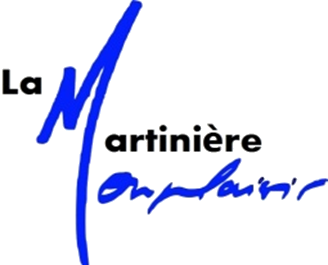
\includegraphics[width=2cm]{png/logo_lycee.png}%
 \end{minipage}}

\fancyhead[C]{\rule{8cm}{.5pt}}

 \fancyhead[R]{%
 \noindent\begin{minipage}[c]{3cm}
 \begin{flushright}
 \footnotesize{\textit{\textsf{\xxtete}}}%
 \end{flushright}
 \end{minipage}
}


\fancyfoot[C]{\rule{12cm}{.5pt}}
\renewcommand{\footrulewidth}{0.2pt}
\fancyfoot[C]{\footnotesize{\bfseries \thepage}}
\fancyfoot[L]{ 
\begin{minipage}[c]{.4\linewidth}
\noindent\footnotesize{{\xxauteur}}
\end{minipage}}


\fancyfoot[R]{\footnotesize{\xxpied}
\ifthenelse{\isodd{\value{page}}}{
\begin{tikzpicture}[overlay]
\node[shape=rectangle, 
      rounded corners = .25 cm,
	  draw= ocre,
	  line width=2pt, 
	  fill = ocre!10,
	  minimum width  = 2.5cm,
	  minimum height = 3cm,] at (\xxposongletx,\xxposonglety) {};
\node at (\xxposonglettext,\xxposonglety) {\rotatebox{90}{\textbf{\large\color{ocre}{\xxonglet}}}};
%{};
\end{tikzpicture}}{}
}
%
%
%
% Removes the header from odd empty pages at the end of chapters
\makeatletter
\renewcommand{\cleardoublepage}{
\clearpage\ifodd\c@page\else
\hbox{}
\vspace*{\fill}
\thispagestyle{empty}
\newpage
\fi}

\fancypagestyle{plain}{%
\fancyhf{} % vide l’en-tête et le pied~de~page.
%\fancyfoot[C]{\bfseries \thepage} % numéro de la page en cours en gras
% et centré en pied~de~page.
\fancyfoot[R]{\footnotesize{\xxpied}}
\fancyfoot[C]{\rule{12cm}{.5pt}}
\renewcommand{\footrulewidth}{0.2pt}
\fancyfoot[C]{\footnotesize{\bfseries \thepage}}
\fancyfoot[L]{ 
\begin{minipage}[c]{.4\linewidth}
\noindent\footnotesize{{\xxauteur}}
\end{minipage}}}



%----------------------------------------------------------------------------------------
%	THEOREM STYLES
%----------------------------------------------------------------------------------------

% Conflit avec la police adobe
%\usepackage{amsmath,amsfonts,amssymb,amsthm} % For math equations, theorems, symbols, etc
\usepackage{amsmath,amsthm}

\newcommand{\intoo}[2]{\mathopen{]}#1\,;#2\mathclose{[}}
\newcommand{\ud}{\mathop{\mathrm{{}d}}\mathopen{}}
\newcommand{\intff}[2]{\mathopen{[}#1\,;#2\mathclose{]}}
%\newtheorem{notation}{Notation}[chapter]
\newtheorem{notation}{Notation}[section]

% Boxed/framed environments
\newtheoremstyle{ocrenumbox}% % Theorem style name
{0pt}% Space above
{0pt}% Space below
{\normalfont}% % Body font
{}% Indent amount
{\small\bf\sffamily\color{ocre}}% % Theorem head font
{\;}% Punctuation after theorem head
{0.25em}% Space after theorem head
{\small\sffamily\color{ocre}\thmname{#1}\nobreakspace\thmnumber%{\@ifnotempty{#1}{}\@upn{#2}}% Theorem text (e.g. Theorem 2.1)
\thmnote{\nobreakspace\the\thm@notefont\sffamily\bfseries\color{black}---\nobreakspace#3.}} % Optional theorem note
\renewcommand{\qedsymbol}{$\blacksquare$}% Optional qed square


% Boite pour les corriges
\newtheoremstyle{correctionbox}% % Theorem style name
{0pt}% Space above
{0pt}% Space below
{\normalfont}% % Body font
{}% Indent amount
{\small\bf\sffamily\color{violet}}% % Theorem head font
{\;}% Punctuation after theorem head
{0.25em}% Space after theorem head
{\small\sffamily\color{ocre}\thmname{#1}\nobreakspace\thmnumber%{\@ifnotempty{#1}{}\@upn{#2}}% Theorem text (e.g. Theorem 2.1)
\thmnote{\nobreakspace\the\thm@notefont\sffamily\bfseries\color{black}---\nobreakspace#3.}} % Optional theorem note
\renewcommand{\qedsymbol}{$\blacksquare$}% Optional qed square



\newtheoremstyle{blacknumex}% Theorem style name
{5pt}% Space above
{5pt}% Space below
{\normalfont}% Body font
{} % Indent amount
{\small\bf\sffamily}% Theorem head font
{\;}% Punctuation after theorem head
{0.25em}% Space after theorem head
{\small\sffamily{\tiny\ensuremath{\blacksquare}}\nobreakspace\thmname{#1}\nobreakspace\thmnumber%{\@ifnotempty{#1}{}\@upn{#2}}% Theorem text (e.g. Theorem 2.1)
\thmnote{\nobreakspace\the\thm@notefont\sffamily\bfseries---\nobreakspace#3.}}% Optional theorem note

\newtheoremstyle{blacknumbox} % Theorem style name
{0pt}% Space above
{0pt}% Space below
{\normalfont}% Body font
{}% Indent amount
{\small\bf\sffamily}% Theorem head font
{\;}% Punctuation after theorem head
{0.25em}% Space after theorem head
{\small\sffamily\thmname{#1}\nobreakspace 
\thmnote{\nobreakspace\the\thm@notefont\sffamily\bfseries---\nobreakspace#3.}}% Optional theorem note

% Non-boxed/non-framed environments
\newtheoremstyle{ocrenum}% % Theorem style name
{5pt}% Space above
{5pt}% Space below
{\normalfont}% % Body font
{}% Indent amount
{\small\bf\sffamily\color{ocre}}% % Theorem head font
{\;}% Punctuation after theorem head
{0.25em}% Space after theorem head
{\small\sffamily\color{ocre}\thmname{#1}\nobreakspace%\thmnumber{\@ifnotempty{#1}{}\@upn{#2}}% Theorem text (e.g. Theorem 2.1)
\thmnote{\nobreakspace\the\thm@notefont\sffamily\bfseries\color{black}---\nobreakspace#3.}} % Optional theorem note
\renewcommand{\qedsymbol}{$\blacksquare$}% Optional qed square
\makeatother

% Environnement pour les titres de parties
\newtheoremstyle{partiebox} 
{0pt}% Space above
{0pt}% Space below
{\normalfont}% Body font
{}% Indent amount
{\small\bf\sffamily}% Theorem head font
{\;}% Punctuation after theorem head
{0.25em}% Space after theorem head




% Defines the theorem text style for each type of theorem to one of the three styles above
\newcounter{dummy} 
\numberwithin{dummy}{section}
\theoremstyle{ocrenumbox}
%\newtheorem{theoremeT}[dummy]{Théorème}
\newtheorem{theoremeT}[dummy]{Théorème}
\newtheorem{resultatT}[dummy]{Résultat}
\newtheorem{savoirT}[dummy]{Savoir}
\newtheorem{methodeT}[dummy]{Méthode}
\newtheorem{objectifT}[dummy]{Objectif}
%\newtheorem{problem}{Problem}[chapter]
\newtheorem{problem}{Problem}[section]
%\newtheorem{exerciseT}{Exercise}[chapter]
\newtheorem{exerciseT}{Exercice}[section]

\theoremstyle{blacknumex}
%\newtheorem{exampleT}{Example}[chapter]
\newtheorem{exempleT}{Exemple}[section]
\newtheorem{termT}{Terminal\\}[section]
\newtheorem{pyT}{Python\\}[section]
\newtheorem{sciT}{Scilab\\}[section]
\newtheorem{pseudoT}{Pseudo Code\\}[section]
\newtheorem{sqlT}{SQL\\}[section]

\theoremstyle{blacknumbox}
%\newtheorem{vocabulary}{Vocabulary}[chapter]
\newtheorem{vocabulary}{Vocabulaire}[section]
%\newtheorem{definitionT}{Definition}[section]
\newtheorem{definitionT}{Définition}[section]
\newtheorem{rappelT}{Rappel}[section]
\newtheorem{demoT}{Démonstration}[section]
\newtheorem{corollaryT}[dummy]{Corollaire}
\newtheorem{hypoT}{Hypothèse(s)}

\theoremstyle{ocrenum}
\newtheorem{proposition}[dummy]{Proposition}

\theoremstyle{partiebox}
\newtheorem{titrepartieT}[]{}
\newtheorem{titrechapitreT}[]{}

\theoremstyle{correctionbox}
\newtheorem{correctionT}[dummy]{\color{violet}{Correction}}

%----------------------------------------------------------------------------------------
%	DEFINITION OF COLORED BOXES
%----------------------------------------------------------------------------------------

\RequirePackage[framemethod=tikz]{mdframed} % Required for creating the theorem, definition, exercise and corollary boxes

% Theorem box
\newmdenv[skipabove=7pt,
skipbelow=7pt,
backgroundcolor=ocre!10,
linecolor=ocre,
innerleftmargin=5pt,
innerrightmargin=5pt,
innertopmargin=5pt,
leftmargin=0cm,
rightmargin=0cm,
innerbottommargin=5pt]{tBox}


% Correction
\newmdenv[skipabove=7pt,
skipbelow=7pt,
backgroundcolor=violet!10,
linecolor=violet,
innerleftmargin=5pt,
innerrightmargin=5pt,
innertopmargin=5pt,
leftmargin=0cm,
rightmargin=0cm,
innerbottommargin=5pt]{coBox}


% Exercise box	  
\newmdenv[skipabove=7pt,
skipbelow=7pt,
rightline=false,
leftline=true,
topline=false,
bottomline=false,
backgroundcolor=ocre!10,
linecolor=ocre,
innerleftmargin=5pt,
innerrightmargin=5pt,
innertopmargin=5pt,
innerbottommargin=5pt,
leftmargin=0cm,
rightmargin=0cm,
linewidth=4pt]{eBox}	

% Definition box
\newmdenv[skipabove=7pt,
skipbelow=7pt,
rightline=false,
leftline=true,
topline=false,
bottomline=false,
backgroundcolor=ocre!10,
linecolor=ocre,
innerleftmargin=5pt,
innerrightmargin=5pt,
innertopmargin=0pt,
leftmargin=0cm,
rightmargin=0cm,
linewidth=4pt,
innerbottommargin=0pt]{dBox}	

% Demonstration box
\newmdenv[skipabove=7pt,
skipbelow=7pt,
rightline=false,
leftline=true,
topline=false,
bottomline=false,
%backgroundcolor=ocre!10,
linecolor=ocre,
innerleftmargin=5pt,
innerrightmargin=5pt,
innertopmargin=0pt,
leftmargin=0cm,
rightmargin=0cm,
linewidth=4pt,
innerbottommargin=0pt]{demoBox}	

% Corollary box
\newmdenv[skipabove=7pt,
skipbelow=7pt,
rightline=false,
leftline=true,
topline=false,
bottomline=false,
linecolor=gray,
backgroundcolor=black!5,
innerleftmargin=5pt,
innerrightmargin=5pt,
innertopmargin=5pt,
leftmargin=0cm,
rightmargin=0cm,
linewidth=4pt,
innerbottommargin=5pt]{cBox}


% Hypothèses
\newmdenv[skipabove=7pt,
skipbelow=7pt,
rightline=false,
leftline=true,
topline=false,
bottomline=false,
linecolor=gray,
backgroundcolor=black!5,
innerleftmargin=5pt,
innerrightmargin=5pt,
innertopmargin=5pt,
leftmargin=0cm,
rightmargin=0cm,
linewidth=4pt,
innerbottommargin=5pt]{hyBox}


% Boite pour le titre de la partie (pBox)
\newmdenv[skipabove=7pt,
skipbelow=7pt,
rightline=true,
leftline=false,
topline=false,
bottomline=false,
linecolor=ocre,
backgroundcolor=none,
innerleftmargin=5pt,
innerrightmargin=5pt,
innertopmargin=5pt,
leftmargin=0cm,
rightmargin=0cm,
linewidth=4pt,
innerbottommargin=5pt]{pBox}

% Boite pour le titre du chapitre (chBox)
\newmdenv[skipabove=7pt,
skipbelow=7pt,
rightline=false,
leftline=true,
topline=false,
bottomline=false,
linecolor=ocre,
%backgroundcolor=black!5,
innerleftmargin=5pt,
innerrightmargin=5pt,
innertopmargin=5pt,
leftmargin=0cm,
rightmargin=0cm,
linewidth=4pt,
innerbottommargin=5pt]{chBox}


% Boite pour les exemples
\newmdenv[skipabove=7pt,
skipbelow=7pt,
rightline=false,
leftline=true,
topline=false,
bottomline=false,
linecolor=gray,
backgroundcolor=white,
innerleftmargin=5pt,
innerrightmargin=5pt,
innertopmargin=5pt,
leftmargin=0cm,
rightmargin=0cm,
linewidth=4pt,
innerbottommargin=5pt]{exBox}

% Boite pour le terminal
\newmdenv[skipabove=7pt,
skipbelow=7pt,
rightline=false,
leftline=true,
topline=false,
bottomline=false,
linecolor=gray,
backgroundcolor=white,
innerleftmargin=5pt,
innerrightmargin=5pt,
innertopmargin=5pt,
leftmargin=0cm,
rightmargin=0cm,
linewidth=4pt,
innerbottommargin=5pt]{termBox}


% Boite pour Python
\newmdenv[skipabove=7pt,
skipbelow=7pt,
rightline=false,
leftline=true,
topline=false,
bottomline=false,
linecolor=gray,
backgroundcolor=white,
innerleftmargin=5pt,
innerrightmargin=5pt,
innertopmargin=0pt,
leftmargin=0cm,
rightmargin=0cm,
linewidth=4pt,
innerbottommargin=5pt]{pyBox}

% Boite pour scilab
\newmdenv[skipabove=7pt,
skipbelow=7pt,
rightline=false,
leftline=true,
topline=false,
bottomline=false,
linecolor=gray,
backgroundcolor=white,
innerleftmargin=5pt,
innerrightmargin=5pt,
innertopmargin=5pt,
leftmargin=0cm,
rightmargin=0cm,
linewidth=4pt,
innerbottommargin=5pt]{sciBox}


% Boite pour pseudo
\newmdenv[skipabove=7pt,
skipbelow=7pt,
rightline=false,
leftline=true,
topline=false,
bottomline=false,
linecolor=gray,
backgroundcolor=white,
innerleftmargin=5pt,
innerrightmargin=5pt,
innertopmargin=5pt,
leftmargin=0cm,
rightmargin=0cm,
linewidth=4pt,
innerbottommargin=5pt]{pseudoBox}

% Boite pour pseudo
\newmdenv[skipabove=7pt,
skipbelow=7pt,
rightline=false,
leftline=true,
topline=false,
bottomline=false,
linecolor=gray,
backgroundcolor=white,
innerleftmargin=5pt,
innerrightmargin=5pt,
innertopmargin=5pt,
leftmargin=0cm,
rightmargin=0cm,
linewidth=4pt,
innerbottommargin=5pt]{sqlBox}


% Creates an environment for each type of theorem and assigns it a theorem text style from the "Theorem Styles" section above and a colored box from above
\newenvironment{theorem}{\begin{tBox}\begin{theoremeT}}{\end{theoremeT}\end{tBox}}
\newenvironment{resultat}{\begin{tBox}\begin{resultatT}}{\end{resultatT}\end{tBox}}
\newenvironment{methode}{\begin{tBox}\begin{methodeT}}{\end{methodeT}\end{tBox}}
\newenvironment{savoir}{\begin{tBox}\begin{savoirT}}{\end{savoirT}\end{tBox}}
\newenvironment{obj}{\begin{tBox}\begin{objectifT}}{\end{objectifT}\end{tBox}}
\newenvironment{corrige}{\begin{coBox}\begin{correctionT}}{\end{correctionT}\end{coBox}}
\newenvironment{exercise}{\begin{eBox}\begin{exerciseT}}{\hfill{\color{ocre}\tiny\ensuremath{\blacksquare}}\end{exerciseT}\end{eBox}}				  
\newenvironment{exercice}{\begin{eBox}\begin{exerciseT}}{\hfill{\color{ocre}\tiny\ensuremath{\blacksquare}}\end{exerciseT}\end{eBox}}				  

\newenvironment{definition}{\begin{dBox}\begin{definitionT}}{\end{definitionT}\end{dBox}}	
\newenvironment{rappel}{\begin{dBox}\begin{rappelT}}{\end{rappelT}\end{dBox}}	
\newenvironment{defi}{\begin{dBox}\begin{definitionT}}{\end{definitionT}\end{dBox}}	
\newenvironment{demo}{\begin{demoBox}\begin{demoT}}{\end{demoT}\end{demoBox}}	
%\newenvironment{exemple}{\begin{exempleT}}{\hfill{\tiny\ensuremath{\blacksquare}}\end{exempleT}}		
\newenvironment{corollary}{\begin{cBox}\begin{corollaryT}}{\end{corollaryT}\end{cBox}}
\newenvironment{hypo}{\begin{hyBox}\begin{hypoT}}{\end{hypoT}\end{hyBox}}	\newenvironment{exemple}{\begin{exBox}\begin{exempleT}}{\hfill{\tiny\ensuremath{\blacksquare}}\end{exempleT}\end{exBox}}	
\newenvironment{titrepartie}{\begin{pBox}\begin{titrepartieT}}{\end{titrepartieT}\end{pBox}}	
\newenvironment{titrechapitre}{\begin{chBox}\begin{titrechapitreT}}{\end{titrechapitreT}\end{chBox}}	

\newenvironment{term}{ \begin{termBox}\begin{termT}}{\end{termT}\end{termBox}}
\newenvironment{py}{ \begin{pyBox}\begin{pyT}}{\end{pyT}\end{pyBox}}
\newenvironment{sci}{ \begin{sciBox}\begin{sciT}}{\end{sciT}\end{sciBox}}
\newenvironment{pseudo}{ \begin{pseudoBox}\begin{pseudoT}}{\end{pseudoT}\end{pseudoBox}}
\newenvironment{envsql}{ \begin{sqlBox}\begin{sqlT}}{\end{sqlT}\end{sqlBox}}


%----------------------------------------------------------------------------------------
%	REMARK ENVIRONMENT
%----------------------------------------------------------------------------------------

\newenvironment{remark}{\par\vspace{10pt}\small % Vertical white space above the remark and smaller font size
\begin{list}{}{
\leftmargin=35pt % Indentation on the left
\rightmargin=25pt}\item\ignorespaces % Indentation on the right
\makebox[-2.5pt]{\begin{tikzpicture}[overlay]
\node[draw=ocre!60,line width=1pt,circle,fill=ocre!25,font=\sffamily\bfseries,inner sep=2pt,outer sep=0pt] at (-15pt,0pt){\textcolor{ocre}{R}};\end{tikzpicture}} % Orange R in a circle
\advance\baselineskip -1pt}{\end{list}\vskip5pt} % Tighter line spacing and white space after remark

\newenvironment{rem}{\par\vspace{10pt}\small % Vertical white space above the remark and smaller font size
\begin{list}{}{
\leftmargin=35pt % Indentation on the left
\rightmargin=25pt}\item\ignorespaces % Indentation on the right
\makebox[-2.5pt]{\begin{tikzpicture}[overlay]
\node[draw=ocre!60,line width=1pt,circle,fill=ocre!25,font=\sffamily\bfseries,inner sep=2pt,outer sep=0pt] at (-15pt,0pt){\textcolor{ocre}{R}};\end{tikzpicture}} % Orange R in a circle
\advance\baselineskip -1pt}{\end{list}\vskip5pt} % Tighter line spacing and white space after remark


\newenvironment{warn}{\par\vspace{10pt}\small % Vertical white space above the remark and smaller font size
\begin{list}{}{
\leftmargin=35pt % Indentation on the left
\rightmargin=25pt}\item\ignorespaces % Indentation on the right
\makebox[-2.5pt]{\begin{tikzpicture}[overlay]
\node[draw=red!60,line width=1pt,circle,fill=red!25,font=\sffamily\bfseries,inner sep=2pt,outer sep=0pt] at (-15pt,0pt){\textcolor{black}{!}};\end{tikzpicture}} % Point d'exclamation dans un cercle
\advance\baselineskip -1pt}{\end{list}\vskip5pt} % Tighter line spacing and white space after remark


%----------------------------------------------------------------------------------------
%	SECTION NUMBERING IN THE MARGIN
%----------------------------------------------------------------------------------------
\setcounter{secnumdepth}{3}
\setcounter{tocdepth}{2}



\makeatletter
\renewcommand{\@seccntformat}[1]{\llap{\textcolor{ocre}{\csname the#1\endcsname}\hspace{1em}}}                    
\renewcommand{\section}{\@startsection{section}{1}{\z@}
{-4ex \@plus -1ex \@minus -.4ex}
{1ex \@plus.2ex }
{\normalfont\large\sffamily\bfseries}}
\renewcommand{\subsection}{\@startsection {subsection}{2}{\z@}
{-3ex \@plus -0.1ex \@minus -.4ex}
{0.5ex \@plus.2ex }
{\normalfont\sffamily\bfseries}}
\renewcommand{\subsubsection}{\@startsection {subsubsection}{3}{\z@}
{-2ex \@plus -0.1ex \@minus -.2ex}
{.2ex \@plus.2ex }
{\normalfont\small\sffamily\bfseries}}                        
\renewcommand\paragraph{\@startsection{paragraph}{4}{\z@}
{-2ex \@plus-.2ex \@minus .2ex}
{.1ex}
{\normalfont\small\sffamily\bfseries}}

%----------------------------------------------------------------------------------------
%	PART HEADINGS
%----------------------------------------------------------------------------------------


%----------------------------------------------------------------------------------------
%	CHAPTER HEADINGS
%----------------------------------------------------------------------------------------

% \newcommand{\thechapterimage}{}%
% \newcommand{\chapterimage}[1]{\renewcommand{\thechapterimage}{#1}}%
% \def\@makechapterhead#1{%
% {\parindent \z@ \raggedright \normalfont
% \ifnum \c@secnumdepth >\m@ne
% \if@mainmatter
% \begin{tikzpicture}[remember picture,overlay]
% \node at (current page.north west)
% {\begin{tikzpicture}[remember picture,overlay]
% \node[anchor=north west,inner sep=0pt] at (0,0) {\includegraphics[width=\paperwidth]{\thechapterimage}};
% \draw[anchor=west] (\Gm@lmargin,-9cm) node [line width=2pt,rounded corners=15pt,draw=ocre,fill=white,fill opacity=0.5,inner sep=15pt]{\strut\makebox[22cm]{}};
% \draw[anchor=west] (\Gm@lmargin+.3cm,-9cm) node {\huge\sffamily\bfseries\color{black}\thechapter. #1\strut};
% \end{tikzpicture}};
% \end{tikzpicture}
% \else
% \begin{tikzpicture}[remember picture,overlay]
% \node at (current page.north west)
% {\begin{tikzpicture}[remember picture,overlay]
% \node[anchor=north west,inner sep=0pt] at (0,0) {\includegraphics[width=\paperwidth]{\thechapterimage}};
% \draw[anchor=west] (\Gm@lmargin,-9cm) node [line width=2pt,rounded corners=15pt,draw=ocre,fill=white,fill opacity=0.5,inner sep=15pt]{\strut\makebox[22cm]{}};
% \draw[anchor=west] (\Gm@lmargin+.3cm,-9cm) node {\huge\sffamily\bfseries\color{black}#1\strut};
% \end{tikzpicture}};
% \end{tikzpicture}
% \fi\fi\par\vspace*{270\p@}}}

%-------------------------------------------

\def\@makeschapterhead#1{%
\begin{tikzpicture}[remember picture,overlay]
\node at (current page.north west)
{\begin{tikzpicture}[remember picture,overlay]
\node[anchor=north west,inner sep=0pt] at (0,0) {\includegraphics[width=\paperwidth]{\thechapterimage}};
\draw[anchor=west] (\Gm@lmargin,-9cm) node [line width=2pt,rounded corners=15pt,draw=ocre,fill=white,fill opacity=0.5,inner sep=15pt]{\strut\makebox[22cm]{}};
\draw[anchor=west] (\Gm@lmargin+.3cm,-9cm) node {\huge\sffamily\bfseries\color{black}#1\strut};
\end{tikzpicture}};
\end{tikzpicture}
\par\vspace*{270\p@}}
\makeatother

%----------------------------------------------------------------------------------------
%	HYPERLINKS IN THE DOCUMENTS
%----------------------------------------------------------------------------------------


\hypersetup{hidelinks,backref=true,pagebackref=true,hyperindex=true,colorlinks=false,breaklinks=true,urlcolor= ocre,bookmarks=true,bookmarksopen=false,pdftitle={Title},pdfauthor={Author}}
\usepackage{bookmark}
\bookmarksetup{
open,
numbered,
addtohook={%
\ifnum\bookmarkget{level}=0 % chapter
\bookmarksetup{bold}%
\fi
\ifnum\bookmarkget{level}=-1 % part
\bookmarksetup{color=ocre,bold}%
\fi
}
}

%----------------------------------------------------------------------------------------
%	
%----------------------------------------------------------------------------------------

\newcommand{\thechapterimage}{}%
\newcommand{\chapterimage}[1]{\renewcommand{\thechapterimage}{#1}}%
\def\@makechapterhead#1{%
{\parindent \z@ \raggedright \normalfont
\begin{tikzpicture}[remember picture,overlay]
\node at (current page.north west)
{\begin{tikzpicture}[remember picture,overlay]
\node[anchor=north west,inner sep=0pt] at (0,0) {\includegraphics[width=\paperwidth]{\thechapterimage}};
%\draw[anchor=west] (\Gm@lmargin,-9cm) node [line width=2pt,rounded corners=15pt,draw=ocre,fill=white,fill opacity=0.5,inner sep=15pt]{\strut\makebox[22cm]{}};
%\draw[anchor=west] (\Gm@lmargin+.3cm,-9cm) node {\huge\sffamily\bfseries\color{black}\thechapter. #1\strut};
\end{tikzpicture}};
\end{tikzpicture}
\par\vspace*{270\p@}
}}

 \newcounter{exo}


\makeatletter             
\renewcommand{\subparagraph}{\@startsection{exo}{5}{\z@}%
                                    {-2ex \@plus-.2ex \@minus .2ex}%
                                    {0ex}%               
{\normalfont\bfseries Question \hspace{.7cm} }}
\makeatother
\renewcommand{\thesubparagraph}{\arabic{subparagraph}} 
\makeatletter


%%%% Environnement pour inclure du code
\usepackage{textcomp}
\usepackage[french]{algorithm2e}
\usepackage{listings}
\lstloadlanguages{R}   % pour regler les pb d accent utf8 dans les codes
\lstset{language=R} % pour regler les pb d accent utf8 dans les codes
\renewcommand{\lstlistlistingname}{Listings}
\renewcommand{\lstlistingname}{Listing}

\SetKwBlock{Fonction}{Début Fonction}{Fin Fonction}
\SetKwComment{Comment}{start}{end}

\definecolor{Bleu}{rgb}{0.1,0.1,1.0}
\definecolor{Noir}{rgb}{0,0,0}
\definecolor{Grau}{rgb}{0.5,0.5,0.5}
\definecolor{DunkelGrau}{rgb}{0.15,0.15,0.15}
\definecolor{Hellbraun}{rgb}{0.5,0.25,0.0}
\definecolor{Magenta}{rgb}{1.0,0.0,1.0}
\definecolor{Gris}{gray}{0.5}
\definecolor{Vert}{rgb}{0,0.5,0}
\definecolor{SourceHintergrund}{rgb}{1,1.0,0.95}


\lstnewenvironment{python}[1][]{
\lstset{
%escapeinside={\%*}{*)},
inputencoding=utf8,   % pour regler les pb d accent utf8 dans les codes
extendedchars=true,   % pour regler les pb d accent utf8 dans les codes
language=python,
basicstyle=\ttfamily\footnotesize, 	
stringstyle=\color{red}, 
showstringspaces=false, 
alsoletter={1234567890},
otherkeywords={\ , \}, \{},
keywordstyle=\color{blue},
emph={access,and,break,class,continue,def,del,elif ,else,
except,exec,finally,for,from,global,if,import,in,i s,
lambda,not,or,pass,print,raise,return,try,while},
emphstyle=\color{black}\bfseries,
emph={[2]True, False, None, self},
emphstyle=[2]\color{black},
emph={[3]from, import, as},
emphstyle=[3]\color{blue},
upquote=true,
columns=flexible, % pour empecher d'avoir un espacement mono
morecomment=[s]{"""}{"""},
commentstyle=\color{Hellbraun}\slshape, 
%emph={[4]1, 2, 3, 4, 5, 6, 7, 8, 9, 0},
emphstyle=[4]\color{blue},
literate=*{:}{{\textcolor{blue}:}}{1}
{=}{{\textcolor{blue}=}}{1}
{-}{{\textcolor{blue}-}}{1}
{+}{{\textcolor{blue}+}}{1}
{*}{{\textcolor{blue}*}}{1}
{!}{{\textcolor{blue}!}}{1}
{(}{{\textcolor{blue}(}}{1}
{)}{{\textcolor{blue})}}{1}
{[}{{\textcolor{blue}[}}{1}
{]}{{\textcolor{blue}]}}{1}
{<}{{\textcolor{blue}<}}{1}
{>}{{\textcolor{blue}>}}{1}
{COMPLETER}{{\textcolor{red}COMPLETER}}{1},
literate=%
            {é}{{\'{e}}}1
            {è}{{\`{e}}}1
            {ê}{{\^{e}}}1
            {ë}{{\¨{e}}}1
            {û}{{\^{u}}}1
            {ù}{{\`{u}}}1
            {â}{{\^{a}}}1
            {à}{{\`{a}}}1
            {î}{{\^{i}}}1
            {ç}{{\c{c}}}1
            {Ç}{{\c{C}}}1
            {É}{{\'{E}}}1
            {Ê}{{\^{E}}}1
            {À}{{\`{A}}}1
            {Â}{{\^{A}}}1
            {Î}{{\^{I}}}1, % pour regler les pb d accent utf8 dans les codes
%framexleftmargin=1mm, framextopmargin=1mm, frame=shadowbox, rulesepcolor=\color{blue},#1
%backgroundcolor=\color{SourceHintergrund}, 
%framexleftmargin=1mm, framexrightmargin=1mm, framextopmargin=1mm, frame=single, framerule=1pt, rulecolor=\color{black},#1
}}{}



\lstnewenvironment{scilab}[1][]{
\lstset{
language=scilab,
basicstyle=\sffamily\footnotesize, 	
stringstyle=\color{red}, 
showstringspaces=false, 
alsoletter={1234567890},
otherkeywords={\ , \}, \{},
keywordstyle=\color{blue},
emph={access,and,break,class,continue,def,del,elif ,else,
except,exec,finally,for,from,global,if,import,in,i s,
lambda,not,or,pass,print,raise,return,try,while,Debut},
emphstyle=\color{black}\bfseries,
emph={[2]True, False, None, self},
emphstyle=[2]\color{black},
emph={[3]from, import, as},
emphstyle=[3]\color{blue},
upquote=true,
columns=flexible, % pour empecher d'avoir un espacement mono
morecomment=[s]{"""}{"""},
commentstyle=\color{Hellbraun}\slshape, 
%emph={[4]1, 2, 3, 4, 5, 6, 7, 8, 9, 0},
emphstyle=[4]\color{blue},
literate=*{:}{{\textcolor{blue}:}}{1}
{=}{{\textcolor{blue}=}}{1}
{-}{{\textcolor{blue}-}}{1}
{+}{{\textcolor{blue}+}}{1}
{*}{{\textcolor{blue}*}}{1}
{!}{{\textcolor{blue}!}}{1}
{(}{{\textcolor{blue}(}}{1}
{)}{{\textcolor{blue})}}{1}
{[}{{\textcolor{blue}[}}{1}
{]}{{\textcolor{blue}]}}{1}
{<}{{\textcolor{blue}<}}{1}
{>}{{\textcolor{blue}>}}{1},
%framexleftmargin=1mm, framextopmargin=1mm, frame=shadowbox, rulesepcolor=\color{blue},#1
%backgroundcolor=\color{SourceHintergrund}, 
%framexleftmargin=1mm, framexrightmargin=1mm, framextopmargin=1mm, frame=single, framerule=1pt, rulecolor=\color{black},#1
}}{}


\lstdefinestyle{stylepython}{%
escapeinside={\%*}{*)},
inputencoding=utf8,   % pour regler les pb d accent utf8 dans les codes
extendedchars=true,   % pour regler les pb d accent utf8 dans les codes
language=python,
basicstyle=\sffamily\footnotesize, 	
stringstyle=\color{red}, 
showstringspaces=false, 
alsoletter={1234567890},
otherkeywords={\ , \}, \{},
keywordstyle=\color{blue},
emph={access,and,break,class,continue,def,del,elif ,else,
except,exec,finally,for,from,global,if,import,in,i s,
lambda,not,or,pass,print,raise,return,try,while},
emphstyle=\color{black}\bfseries,
emph={[2]True, False, None, self},
emphstyle=[2]\color{green},
emph={[3]from, import, as},
emphstyle=[3]\color{blue},
upquote=true,
columns=flexible, % pour empecher d'avoir un espacement mono
morecomment=[s]{"""}{"""},
commentstyle=\color{Hellbraun}\slshape, 
%emph={[4]1, 2, 3, 4, 5, 6, 7, 8, 9, 0},
emphstyle=[4]\color{blue},
literate=*{:}{{\textcolor{blue}:}}{1}
{=}{{\textcolor{blue}=}}{1}
{-}{{\textcolor{blue}-}}{1}
{+}{{\textcolor{blue}+}}{1}
{*}{{\textcolor{blue}*}}{1}
{!}{{\textcolor{blue}!}}{1}
{(}{{\textcolor{blue}(}}{1}
{)}{{\textcolor{blue})}}{1}
{[}{{\textcolor{blue}[}}{1}
{]}{{\textcolor{blue}]}}{1}
{<}{{\textcolor{blue}<}}{1}
{>}{{\textcolor{blue}>}}{1}
{COMPLETER}{{\textcolor{red}COMPLETER}}{1},
literate=%
            {é}{{\'{e}}}1
            {è}{{\`{e}}}1
            {ê}{{\^{e}}}1
            {ë}{{\¨{e}}}1
            {û}{{\^{u}}}1
            {ù}{{\`{u}}}1
            {â}{{\^{a}}}1
            {à}{{\`{a}}}1
            {î}{{\^{i}}}1
            {ç}{{\c{c}}}1
            {Ç}{{\c{C}}}1
            {É}{{\'{E}}}1
            {Ê}{{\^{E}}}1
            {À}{{\`{A}}}1
            {Â}{{\^{A}}}1
            {Î}{{\^{I}}}1,
%numbers=left,                    % where to put the line-numbers; possible values are (none, left, right)
%numbersep=5pt,                   % how far the line-numbers are from the code
%numberstyle=\tiny\color{mygray}, % the style that is used for the line-numbers
}



\lstnewenvironment{termi}[1][]{
\lstset{
language=scilab,
basicstyle=\sffamily\footnotesize, 	
stringstyle=\color{red}, 
showstringspaces=false, 
alsoletter={1234567890},
otherkeywords={\ , \}, \{},
keywordstyle=\color{blue},
emph={access,and,break,class,continue,def,del,elif ,else,
except,exec,finally,for,from,global,if,import,in,i s,
lambda,not,or,pass,print,raise,return,try,while,Debut},
emphstyle=\color{black}\bfseries,
emph={[2]True, False, None, self},
emphstyle=[2]\color{green},
emph={[3]from, import, as},
emphstyle=[3]\color{blue},
upquote=true,
columns=flexible, % pour empecher d'avoir un espacement mono
morecomment=[s]{"""}{"""},
commentstyle=\color{Hellbraun}\slshape, 
%emph={[4]1, 2, 3, 4, 5, 6, 7, 8, 9, 0},
emphstyle=[4]\color{blue},
literate=*{:}{{\textcolor{blue}:}}{1}
{=}{{\textcolor{blue}=}}{1}
{-}{{\textcolor{blue}-}}{1}
{+}{{\textcolor{blue}+}}{1}
{*}{{\textcolor{blue}*}}{1}
{!}{{\textcolor{blue}!}}{1}
{(}{{\textcolor{blue}(}}{1}
{)}{{\textcolor{blue})}}{1}
{[}{{\textcolor{blue}[}}{1}
{]}{{\textcolor{blue}]}}{1}
{<}{{\textcolor{blue}<}}{1}
{>}{{\textcolor{blue}>}}{1},
%framexleftmargin=1mm, framextopmargin=1mm, frame=shadowbox, rulesepcolor=\color{blue},#1
%backgroundcolor=\color{SourceHintergrund}, 
%framexleftmargin=1mm, framexrightmargin=1mm, framextopmargin=1mm, frame=single, framerule=1pt, rulecolor=\color{black},#1
}}{}


\lstnewenvironment{sql}[1][]{
\lstset{
%escapeinside={\%*}{*)},
%inputencoding=utf8,   % pour regler les pb d accent utf8 dans les codes
%extendedchars=true,   % pour regler les pb d accent utf8 dans les codes
language=sql,
basicstyle=\sffamily\footnotesize, 	
stringstyle=\color{red}, 
showstringspaces=false, 
alsoletter={1234567890},
otherkeywords={\ , \}, \{},
keywordstyle=\color{blue},
emph={access,and,break,class,continue,def,del,elif ,else,
except,exec,finally,for,from,global,if,import,in,i s,
lambda,not,or,pass,print,raise,return,try,while},
emphstyle=\color{black}\bfseries,
emph={[2]True, False, None, self},
emphstyle=[2]\color{black},
emph={[3]from, import, as},
emphstyle=[3]\color{blue},
upquote=true,
columns=flexible, % pour empecher d'avoir un espacement mono
morecomment=[s]{"""}{"""},
commentstyle=\color{Hellbraun}\slshape, 
%emph={[4]1, 2, 3, 4, 5, 6, 7, 8, 9, 0},
emphstyle=[4]\color{blue},
literate=*{:}{{\textcolor{blue}:}}{1}
{=}{{\textcolor{blue}=}}{1}
{-}{{\textcolor{blue}-}}{1}
{+}{{\textcolor{blue}+}}{1}
{*}{{\textcolor{blue}*}}{1}
{!}{{\textcolor{blue}!}}{1}
{(}{{\textcolor{blue}(}}{1}
{)}{{\textcolor{blue})}}{1}
{[}{{\textcolor{blue}[}}{1}
{]}{{\textcolor{blue}]}}{1}
{<}{{\textcolor{blue}<}}{1}
{>}{{\textcolor{blue}>}}{1}
{COMPLETER}{{\textcolor{red}COMPLETER}}{1},
literate=%
            {é}{{\'{e}}}1
            {è}{{\`{e}}}1
            {ê}{{\^{e}}}1
            {ë}{{\¨{e}}}1
            {û}{{\^{u}}}1
            {ù}{{\`{u}}}1
            {â}{{\^{a}}}1
            {à}{{\`{a}}}1
            {î}{{\^{i}}}1
            {ç}{{\c{c}}}1
            {Ç}{{\c{C}}}1
            {É}{{\'{E}}}1
            {Ê}{{\^{E}}}1
            {À}{{\`{A}}}1
            {Â}{{\^{A}}}1
            {Î}{{\^{I}}}1, % pour regler les pb d accent utf8 dans les codes
%framexleftmargin=1mm, framextopmargin=1mm, frame=shadowbox, rulesepcolor=\color{blue},#1
%backgroundcolor=\color{SourceHintergrund}, 
%framexleftmargin=1mm, framexrightmargin=1mm, framextopmargin=1mm, frame=single, framerule=1pt, rulecolor=\color{black},#1
}}{}


% Définition des booleéns
\newif\iffiche
\newif\ifprof
\newif\iftd
\newif\ifcours

%%%%%%%%%%%%
% Définition des vecteurs 
%%%%%%%%%%%%
 \newcommand{\vect}[1]{\overrightarrow{#1}}
\newcommand{\axe}[2]{\left(#1,\vect{#2}\right)}

\newcommand{\rep}[1]{\mathcal{R}_{#1}}
\newcommand{\vx}[1]{\vect{x_{#1}}}
\newcommand{\vy}[1]{\vect{y_{#1}}}
\newcommand{\vz}[1]{\vect{z_{#1}}}

%%%%%%%%%%%%
% Définition des torseurs 
%%%%%%%%%%%%

 \newcommand{\torseur}[1]{%
\left\{{#1}\right\}
}

\newcommand{\torseurcin}[3]{%
\left\{\mathcal{#1} \left(#2/#3 \right) \right\}
}

\newcommand{\torseurstat}[3]{%
\left\{\mathcal{#1} \left(#2\rightarrow #3 \right) \right\}
}

 \newcommand{\torseurc}[8]{%
%\left\{#1 \right\}=
\left\{
{#1}
\right\}
 = 
\left\{%
\begin{array}{cc}%
{#2} & {#5}\\%
{#3} & {#6}\\%
{#4} & {#7}\\%
\end{array}%
\right\}_{#8}%
}

 \newcommand{\torseurcol}[7]{
\left\{%
\begin{array}{cc}%
{#1} & {#4}\\%
{#2} & {#5}\\%
{#3} & {#6}\\%
\end{array}%
\right\}_{#7}%
}

 \newcommand{\torseurl}[3]{%
%\left\{\mathcal{#1}\right\}_{#2}=%
\left\{%
\begin{array}{l}%
{#1} \\%
{#2} %
\end{array}%
\right\}_{#3}%
}

 \newcommand{\vectv}[3]{%
\vect{V\left( {#1} \in {#2}/{#3}\right)}
}


\newcommand{\vectf}[2]{%
\vect{R\left( {#1} \rightarrow {#2}\right)}
}

\newcommand{\vectm}[3]{%
\vect{\mathcal{M}\left( {#1}, {#2} \rightarrow {#3}\right)}
}


 \newcommand{\vectg}[3]{%
\vect{\Gamma \left( {#1} \in {#2}/{#3}\right)}
}

 \newcommand{\vecto}[2]{%
\vect{\Omega\left( {#1}/{#2}\right)}
}
% }$$\left\{\mathcal{#1} \right\}_{#2} =%
% \left\{%
% \begin{array}{c}%
%  #3 \\%
%  #4 %
% \end{array}%
% \right\}_{#5}}

%\fichetrue
%\fichefalse

%\proftrue
\proffalse

%\tdtrue
\tdfalse

\courstrue
%\coursfalse

% -------------------------------------
% Déclaration des titres
% -------------------------------------

\def\discipline{Sciences \\Industrielles de \\ l'Ingénieur}
\def\xxtete{Sciences Industrielles de l'Ingénieur}

\def\classe{PTSI}
\def\xxnumpartie{Partie 2}
\def\xxpartie{Découverte des Systèmes Linéaires Continus et Invariants\\
Analyse, Modélisation, Résolution}

\def\xxnumchapitre{Chapitre 1}
\def\xxchapitre{\hspace{.12cm} Introduction aux Systèmes Linéaires Continus Invariants}

\def\xxposongletx{2}
\def\xxposonglettext{1.45}
\def\xxposonglety{23}
\def\xxonglet{Part. 2 -- Ch. 1}

\def\xxactivite{Cours}
\def\xxauteur{\textsl{Xavier Pessoles}}

\def\xxcompetences{%
\textsl{%
\textbf{Savoirs et compétences :}
\begin{itemize}[label=\ding{112},font=\color{ocre}] 
\item A-C11.1 : Définition et structure d'un système asservi : chaîne directe (ou chaîne d'action), chaîne de retour (ou chaîne d'acquisition), comparateur et écart.
\item A-C11.2 : Consigne, perturbation.
\item A-C11.3 : Régulation, poursuite.
\item A-C11.4 : Définition des performances : rapidité, précision et stabilité. 
\end{itemize}
%
}}

\def\xxfigures{
\begin{center}
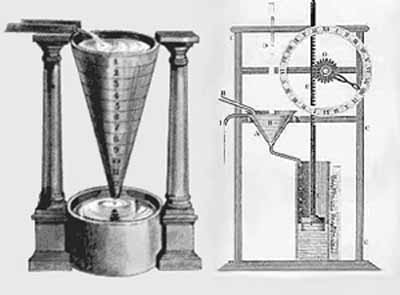
\includegraphics[width=.6\textwidth]{images/clock}

\textit{Horloge à eau (II\ieme s. av. J.C.)}

\rotatebox{270}{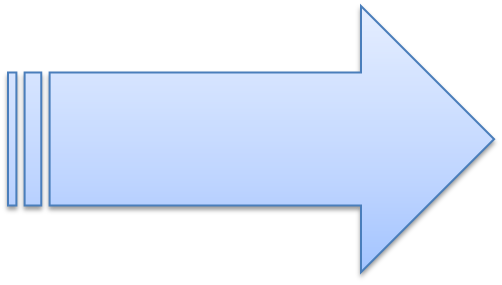
\includegraphics[width=.4\textwidth]{images/fleche}}

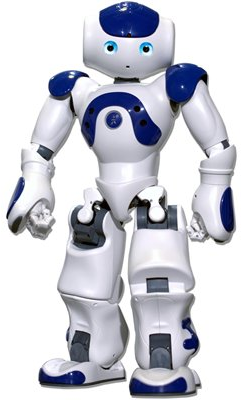
\includegraphics[width=.4\textwidth]{images/nao}

\textit{Robot Nao (XXI\ieme s.)}
\end{center}
}%figues de la page de garde
\def\xxpied{%
Partie 1 -- Découverte des SLCI\\
Ch. 1 : Introduction aux SLCI -- \xxactivite%
}

%---------------------------------------------------------------------------


\begin{document}
\chapterimage{images/Fond_SLCI}
\pagestyle{empty}


%%%%%%%% PAGE DE GARDE COURS
\ifcours
\begin{tikzpicture}[remember picture,overlay]
\node at (current page.north west)
{\begin{tikzpicture}[remember picture,overlay]
\node[anchor=north west,inner sep=0pt] at (0,0) {\includegraphics[width=\paperwidth]{\thechapterimage}};
\draw[anchor=west] (-2cm,-8cm) node [line width=2pt,rounded corners=15pt,draw=ocre,fill=white,fill opacity=0.6,inner sep=40pt]{\strut\makebox[22cm]{}};
\draw[anchor=west] (1cm,-8cm) node {\huge\sffamily\bfseries\color{black} %
\begin{minipage}{1cm}
\rotatebox{90}{\LARGE\sffamily\textsc{\color{ocre}\textbf{\xxnumpartie}}}
\end{minipage} \hfill
\begin{minipage}[c]{14cm}
\begin{titrepartie}
\begin{flushright}
\renewcommand{\baselinestretch}{1.1} 
\Large\sffamily\textsc{\textbf{\xxpartie}}
\renewcommand{\baselinestretch}{1} 
\end{flushright}
\end{titrepartie}
\end{minipage} \hfill
\begin{minipage}[c]{3.5cm}
{\large\sffamily\textsc{\textbf{\color{ocre} \discipline}}}
\end{minipage} 
 };
\end{tikzpicture}};
\end{tikzpicture}


\begin{tikzpicture}[overlay]
\node[shape=rectangle, 
      rounded corners = .25 cm,
	  draw= ocre,
	  line width=2pt, 
	  fill = ocre!10,
	  minimum width  = 2.5cm,
	  minimum height = 3cm,] at (18cm,0) {};
\node at (17.7cm,0) {\rotatebox{90}{\textbf{\Large\color{ocre}{\classe}}}};
%{};
\end{tikzpicture}

\vspace{3.5cm}

\begin{tikzpicture}[remember picture,overlay]
\draw[anchor=west] (-2cm,-6cm) node {\huge\sffamily\bfseries\color{black} %
\begin{minipage}{2cm}
\begin{center}
\LARGE\sffamily\textsc{\color{ocre}\textbf{\xxactivite}}
\end{center}
\end{minipage} \hfill
\begin{minipage}[c]{15cm}
\begin{titrechapitre}
\renewcommand{\baselinestretch}{1.1} 
\Large\sffamily\textsc{\textbf{\xxnumchapitre}}

\Large\sffamily\textsc{\textbf{\xxchapitre}}
\vspace{.5cm}

\renewcommand{\baselinestretch}{1} 
\normalsize\normalfont
\xxcompetences
\end{titrechapitre}
\end{minipage}  };
\end{tikzpicture}
\vfill

\begin{flushright}
\begin{minipage}[c]{.3\linewidth}
\begin{center}
\xxfigures
\end{center}
\end{minipage}\hfill
\begin{minipage}[c]{.6\linewidth}
\startcontents
\printcontents{}{1}{}
\end{minipage}
\end{flushright}

\begin{tikzpicture}[remember picture,overlay]
\draw[anchor=west] (4.5cm,-.7cm) node {
\begin{minipage}[c]{.2\linewidth}
\begin{flushright}

\includegraphics[width=2cm]{png/logoCC}
\end{flushright}
\end{minipage}
\begin{minipage}[c]{.2\linewidth}
\textsl{\xxauteur} \\
\textsl{\classe}
\end{minipage}
 };
\end{tikzpicture}
\newpage
\pagestyle{fancy}

\newpage
\pagestyle{fancy}

\else
\fi


%%%%%%%% PAGE DE GARDE TD
\iftd
%\begin{tikzpicture}[remember picture,overlay]
%\node at (current page.north west)
%{\begin{tikzpicture}[remember picture,overlay]
%\draw[anchor=west] (-2cm,-3.25cm) node [line width=2pt,rounded corners=15pt,draw=ocre,fill=white,fill opacity=0.6,inner sep=40pt]{\strut\makebox[22cm]{}};
%\draw[anchor=west] (1cm,-3.25cm) node {\huge\sffamily\bfseries\color{black} %
%\begin{minipage}{1cm}
%\rotatebox{90}{\LARGE\sffamily\textsc{\color{ocre}\textbf{\xxnumpartie}}}
%\end{minipage} \hfill
%\begin{minipage}[c]{13.5cm}
%\begin{titrepartie}
%\begin{flushright}
%\renewcommand{\baselinestretch}{1.1} 
%\Large\sffamily\textsc{\textbf{\xxpartie}}
%\renewcommand{\baselinestretch}{1} 
%\end{flushright}
%\end{titrepartie}
%\end{minipage} \hfill
%\begin{minipage}[c]{3.5cm}
%{\large\sffamily\textsc{\textbf{\color{ocre} \discipline}}}
%\end{minipage} 
% };
%\end{tikzpicture}};
%\end{tikzpicture}

%%%%%%%%%% PAGE DE GARDE TD %%%%%%%%%%%%%%%
%\begin{tikzpicture}[overlay]
%\node[shape=rectangle, 
%      rounded corners = .25 cm,
%	  draw= ocre,
%	  line width=2pt, 
%	  fill = ocre!10,
%	  minimum width  = 2.5cm,
%	  minimum height = 2.5cm,] at (18.5cm,0) {};
%\node at (17.7cm,0) {\rotatebox{90}{\textbf{\Large\color{ocre}{\classe}}}};
%%{};
%\end{tikzpicture}

% PARTIE ET CHAPITRE
%\begin{tikzpicture}[remember picture,overlay]
%\draw[anchor=west] (-1cm,-2.1cm) node {\large\sffamily\bfseries\color{black} %
%\begin{minipage}[c]{15cm}
%\begin{flushleft}
%\xxnumchapitre \\
%\xxchapitre
%\end{flushleft}
%\end{minipage}  };
%\end{tikzpicture}

% Bandeau titre exo
\begin{tikzpicture}[remember picture,overlay]
\draw[anchor=west] (-2cm,-6cm) node {\huge\sffamily\bfseries\color{black} %
\begin{minipage}{5cm}
\begin{center}
\LARGE\sffamily\color{ocre}\textbf{\textsc{\xxactivite}}

\begin{center}
\xxfigures
\end{center}

\end{center}
\end{minipage} \hfill
\begin{minipage}[c]{12cm}
\begin{titrechapitre}
\renewcommand{\baselinestretch}{1.1} 
\large\sffamily\textbf{\textsc{\xxtitreexo}}

\small\sffamily{\textbf{\textit{\color{black!70}\xxsourceexo}}}
\vspace{.5cm}

\renewcommand{\baselinestretch}{1} 
\normalsize\normalfont
\xxcompetences
\end{titrechapitre}
\end{minipage}  };
\end{tikzpicture}

\else
\fi


%%%%%%%% PAGE DE GARDE FICHE
\iffiche
\begin{tikzpicture}[remember picture,overlay]
\node at (current page.north west)
{\begin{tikzpicture}[remember picture,overlay]
\draw[anchor=west] (-2cm,-3.25cm) node [line width=2pt,rounded corners=15pt,draw=ocre,fill=white,fill opacity=0.6,inner sep=40pt]{\strut\makebox[22cm]{}};
\draw[anchor=west] (1cm,-3.25cm) node {\huge\sffamily\bfseries\color{black} %
\begin{minipage}{1cm}
\rotatebox{90}{\LARGE\sffamily\textsc{\color{ocre}\textbf{\xxnumpartie}}}
\end{minipage} \hfill
\begin{minipage}[c]{14cm}
\begin{titrepartie}
\begin{flushright}
\renewcommand{\baselinestretch}{1.1} 
\large\sffamily\textsc{\textbf{\xxpartie} \\} 

\vspace{.2cm}

\normalsize\sffamily\textsc{\textbf{\xxnumchapitre -- \xxchapitre}}
\renewcommand{\baselinestretch}{1} 
\end{flushright}
\end{titrepartie}
\end{minipage} \hfill
\begin{minipage}[c]{3.5cm}
{\large\sffamily\textsc{\textbf{\color{ocre} \discipline}}}
\end{minipage} 
 };
\end{tikzpicture}};
\end{tikzpicture}


\begin{tikzpicture}[overlay]
\node[shape=rectangle, 
      rounded corners = .25 cm,
	  draw= ocre,
	  line width=2pt, 
	  fill = ocre!10,
	  minimum width  = 2.5cm,
	  minimum height = 2.5cm,] at (18.5cm,0.5cm) {};
%	  minimum height = 2.5cm,] at (18.5cm,0cm) {};
\node at (17.7cm,0.5) {\rotatebox{90}{\textsf{\textbf{\large\color{ocre}{\classe}}}}};
%{};
\end{tikzpicture}



\else
\fi




%\newpage

%
%
%
%
%\vspace{.5cm}
%
%
%\begin{minipage}[c]{.4\linewidth}
%\begin{center}
%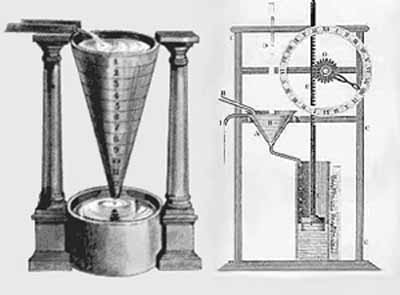
\includegraphics[width=.9\textwidth]{images/clock}
%
%\textit{Horloge à eau (II\ieme s. av. J.C.)}
%\end{center}
%\end{minipage}\hfill
%\begin{minipage}[c]{.2\linewidth}
%\begin{center}
%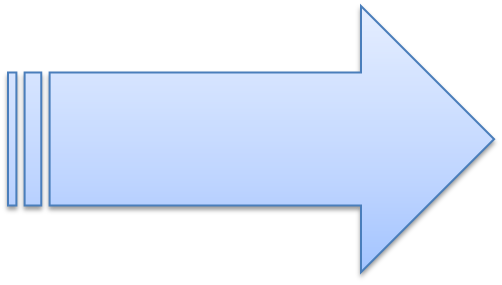
\includegraphics[width=.8\textwidth]{images/fleche}
%\end{center}
%\end{minipage}\hfill
%\begin{minipage}[c]{.25\linewidth}
%\begin{center}
%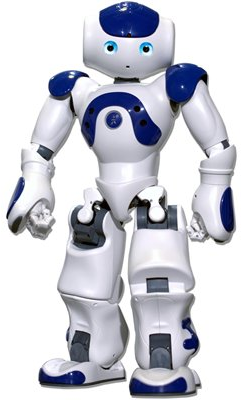
\includegraphics[width=\textwidth]{images/nao}
%
%\textit{Robot Nao (XXI\ieme s.)}
%\end{center}
%\end{minipage}
%%\includegraphics[width=.4\textwidth]{images/renault_frendzy}
%
%
%
%\vspace{.2cm}
%
%Depuis l'antiquité les Hommes cherchent à automatiser différentes tâches du quotidien. 
%\begin{itemize}
%\item Quelle a été l'évolution des systèmes automatisés au cours du temps ?
%\item Quelles sont les caractéristiques des systèmes automatisés ?
%\end{itemize}
%
%
%\begin{savoir}
%\begin{itemize}
%\item A-C11.1 : Définition et structure d'un système asservi : chaîne directe (ou chaîne d'action), chaîne de retour (ou chaîne d'acquisition), comparateur et écart.
%\item A-C11.2 : Consigne, perturbation.
%\item A-C11.3 : Régulation, poursuite.
%\item A-C11.4 : Définition des performances : rapidité, précision et stabilité.
%\end{itemize}
%\end{savoir}
%
%%
%%\begin{rem}
%%\textsc{Savoirs :}
%%\begin{itemize}
%%\item Définir ce qu'est un système asservi
%%\item Définir la nature des informations
%%\item Définir les performances d'un système
%%\end{itemize}
%%\end{rem}
%
%
%\setlength{\parskip}{0ex plus 0.2ex minus 0ex}
% \renewcommand{\contentsname}{}
% \renewcommand{\baselinestretch}{1}
%
%% \vspace{1cm}
%\textit{Ce document est en évolution permanente. Merci de signaler toutes
%erreurs ou coquilles.}
%
%\tableofcontents
%
% \renewcommand{\baselinestretch}{1.2}
%\setlength{\parskip}{2ex plus 0.5ex minus 0.2ex}
%

%

%


%%%%%%% FIN AVIRER %%%%%%%%%%%%%%%
\section{Historique}
L'automatique a pour origine étymologique le mot grec \textit{automatos} qui
signifie «~qui se meut de soi-même~». Historiquement, cette science est
plutôt née de techniques permettant de mettre en \oe{}vre la régulation de
systèmes.

Très tôt, les hommes ont donc chercher à automatiser des tâches afin
d'améliorer le confort de leur existence ou pour améliorer leur sécurité. Plus
tard, avec l'essor de l'industrie au XIX\ieme siècle, les hommes chercheront à
automatiser les tâches répétitives et délicates afin d'accroître la
productivité et d'améliorer la précision.

\subsection{La mesure du temps}

Dès l'antiquité s'est posé le problème de compter le temps. Dans le but
d'améliorer la précision des clepsydres, Ctésibios d'Alexandrie, en 270 av.
JC développa un système innovant. En s'apercevant que le débit d'un fluide
devenait constant en maintenant une hauteur d'eau constante, il introduit un
réservoir entre la source d'eau et réservoir aval. Un flotteur situé dans ce
dernier et relié à une règle permet de mesurer le temps.

 \begin{center}
 \includegraphics[width=.8\textwidth]{images/clepsydre}
 \end{center}

\subsection{L'automatisation du calcul}
\begin{minipage}[c]{0.7\textwidth}
Pour faciliter le travail de son père, surintendant de Haute Normandie, Pascal
mis au point la Pascaline, machine à calculer qui permettait de réaliser de
façon automatique addition, soustraction et multiplication.  

\end{minipage}\hfill
\begin{minipage}[c]{0.2\textwidth}
 \begin{center}
 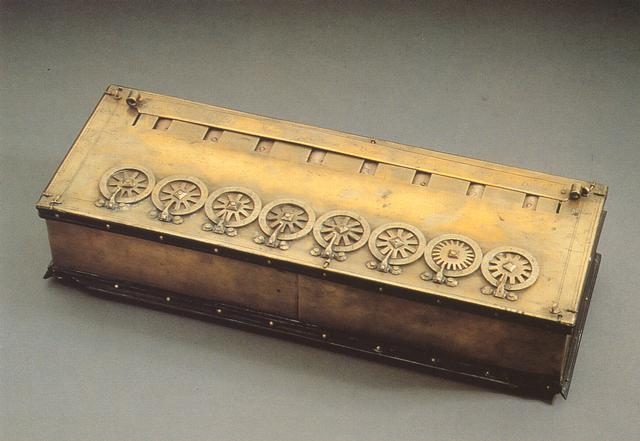
\includegraphics[height=2.5cm]{images/pascal}

\textit{Machine à calculer de Pascal (XVII\ieme s.)}
 \end{center}
\end{minipage}

\subsection{La régulation}

Dans le but de réguler la vitesse de rotation des machines à vapeur, James Watt
fut un des premiers ingénieurs à inventer un mécanisme à rétroaction. 

Il utilisa pour cela un mécanisme rotatif équipé de deux boules reliées à la
sortie d'une machine à vapeur. En tournant, et par le biais des forces
d'inertie, les deux boules étaient animées d'un mouvement d'élévation. Par un
mécanisme de biellettes, l'élévation de ces boules entraînaient une réduction
du débit de vapeur dans la machine à vapeur. 

A l'inverse, lors du ralentissement de la machine, les boules retombaient,
provoquant une augmentation du débit de vapeur dans la machine à vapeur.

\begin{center}
 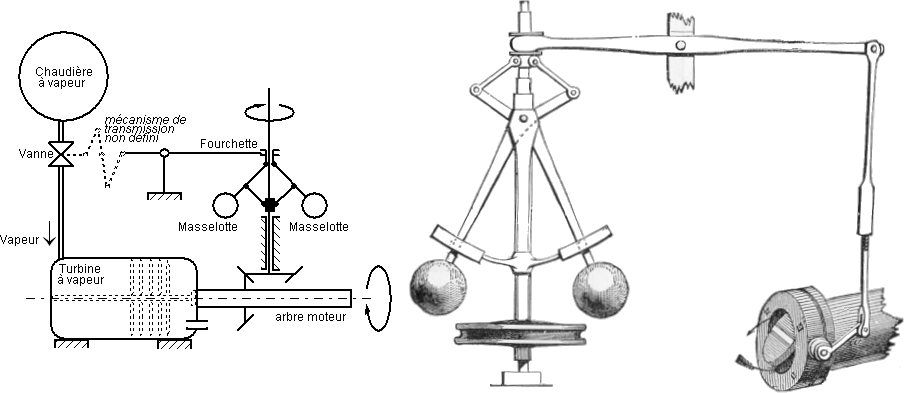
\includegraphics[width=0.8\textwidth]{images/watt}

\textit{Régulateur à boules de Watt (XVIII\ieme s.)}
 \end{center}


\subsection{Les automates}
\begin{minipage}[c]{0.7\textwidth}
La période s'étalant du XVIII\ieme au XIX\ieme siècle est marquée par de
nombreuses créations comme le « canard » de Vaucanson.
Cet ingénieur avait réussi à créer un automate qui ingérait de la nourriture, en
faisait une bouillie, et la rejetait par le postérieur. En outre le canard battait des ailes. 

\end{minipage}\hfill
\begin{minipage}[c]{0.2\textwidth}
 \begin{center}
 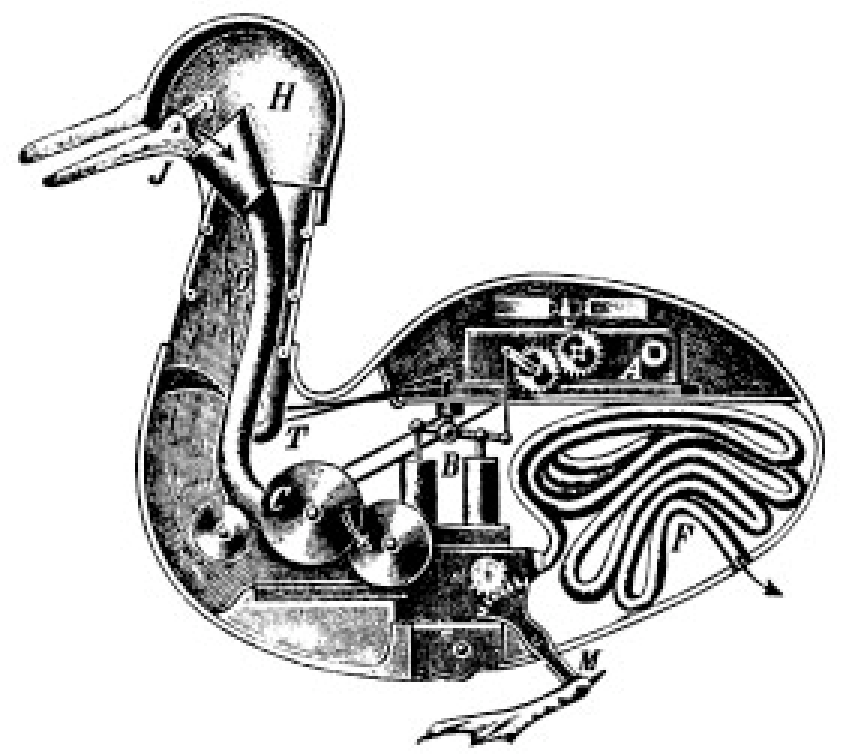
\includegraphics[height=2.5cm]{images/vaucanson}

\textit{Canard digérateur de Vaucanson (XVIII\ieme s.)}
 \end{center}
\end{minipage}

\subsection{L'automatisation des tâches}
\begin{minipage}[c]{0.7\textwidth}
Avec la révolution industrielle au XIX\ieme siècle, l'automatisation des tâches prend de l'ampleur. Dans tous les secteurs industriels, on cherche à accroître la productivité pour faire face à une demande croissante. Dans le domaine du textile en particulier, Jacquard met au point des métiers à tisser semi-automatiques en utilisant des cartes perforées.

\end{minipage}\hfill
\begin{minipage}[c]{0.25\textwidth}
 \begin{center}
 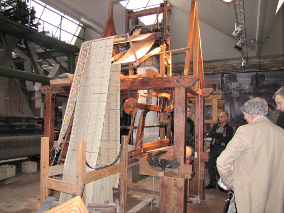
\includegraphics[height=3cm]{images/jacquard_p}

\textit{Métier à tisser -- Jacquard (XIX\ieme s.)}
 \end{center}
\end{minipage}

\subsection{L'arrivée de l'électronique}
\begin{minipage}[c]{0.7\textwidth}
Au fur et à mesure de l'évolution, les tâches se complexifient et le volume des informations à traiter aussi. C'est ainsi qu'au XX\ieme siècle, l'électronique va permettre d'intégrer une grande quantité d'informations et va pouvoir générer un grand nombre de commandes pour des actionneurs différents.
\end{minipage}\hfill
\begin{minipage}[c]{0.2\textwidth}
 \begin{center}
 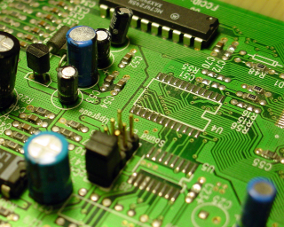
\includegraphics[height=2.5cm]{images/electro_p}
 \end{center}
\end{minipage}

\subsection{La robotique}
\begin{minipage}[c]{0.5\textwidth}
Le début du XXI \ieme siècle voit l'arrivée des premiers robots humanoïdes grands publics. Les problèmes posés par la conception de ces produits provient de la difficulté de reproduire les comportements humains. En effet, il va falloir créer des robots qui ont d'une part des mouvements aussi fluides que les mouvements humains, qui ne doivent pas être déséquilibrés par leur propre poids, qui doivent gérer des situations de chutes, la marche sur des sols glissants.

La robotique reste un domaine de pointe de la recherche française et internationale.
\end{minipage}\hfill
\begin{minipage}[c]{0.4\textwidth}
 \begin{center}
 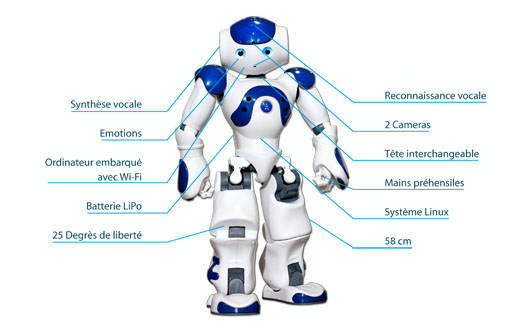
\includegraphics[height=4cm]{images/nao2}

\textit{Robot Nao -- Aldebaran Robotics (XXI\ieme s.)}
 \end{center}
\end{minipage}

\section{Les systèmes automatisés}
\subsection{Présentation}


Les systèmes techniques qui nous entourent peuvent être classés en trois
catégories : 
\begin{itemize}
 \item les \textbf{systèmes manuels} (ou élémentaires) pour lesquels l'intervention humaine prédomine. L'utilisateur commande le système et fournit l'énergie (musculaire) nécessaire à la réalisation de la fonction de service (FS) pour laquelle le système a été conçu;
\item les \textbf{systèmes mécanisés} conçus pour alléger la tâche de l'utilisateur. 
Dans ces systèmes, l'énergie provient le plus souvent d'une source extérieure et le rôle de l'utilisateur consiste à commander le système;
\item les \textbf{systèmes automatisés} pour lesquels l'intervention humaine se
limite à la programmation du système et à son réglage préalable.
\end{itemize}


\begin{exemple}
  Fonction de service : voler dans l'air
  
  
\begin{center}
 \begin{tabular}{ccc}
  \multicolumn{3}{c}{FS : Voler dans l'air} \\
  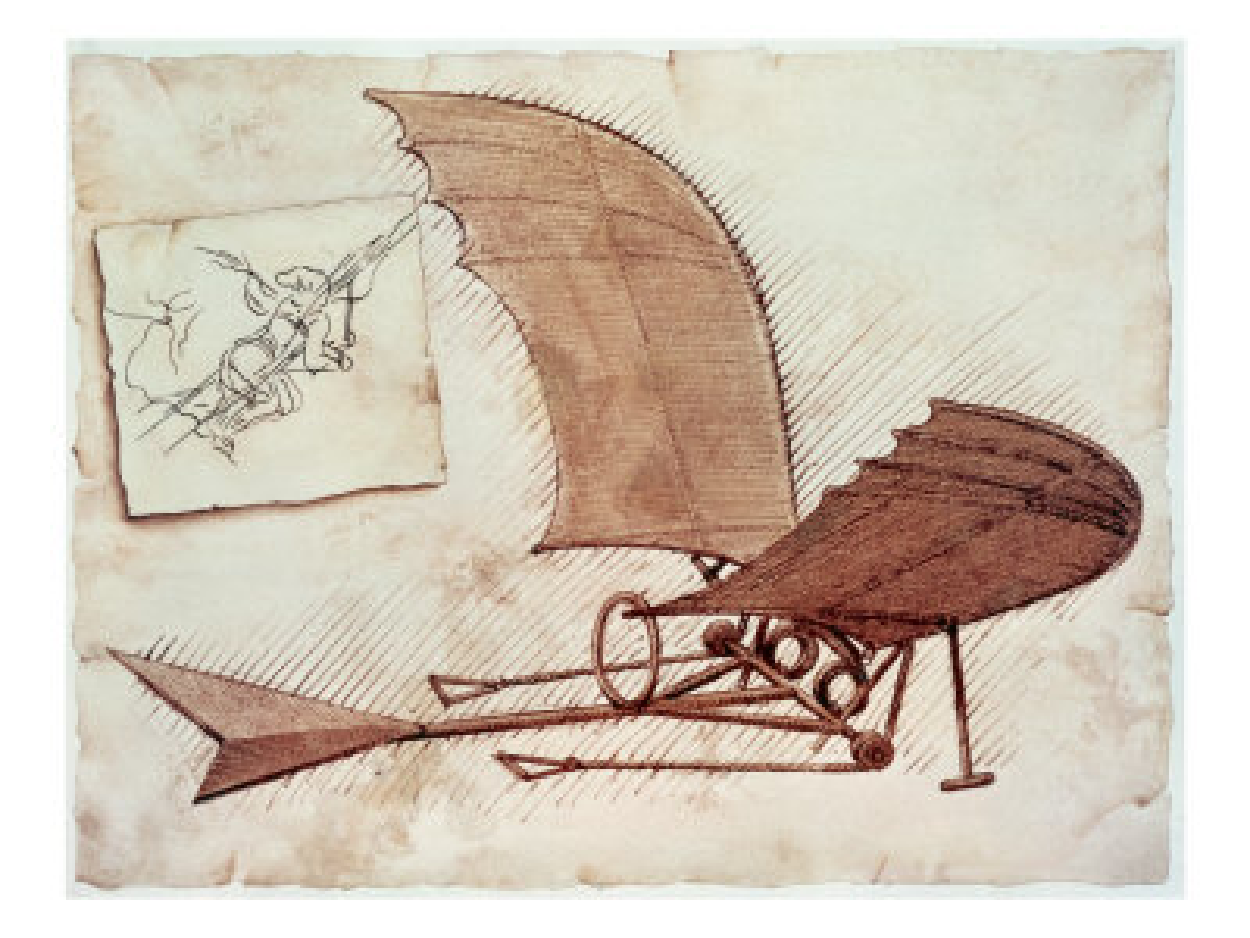
\includegraphics[height=3cm]{images/machineLDV} &
  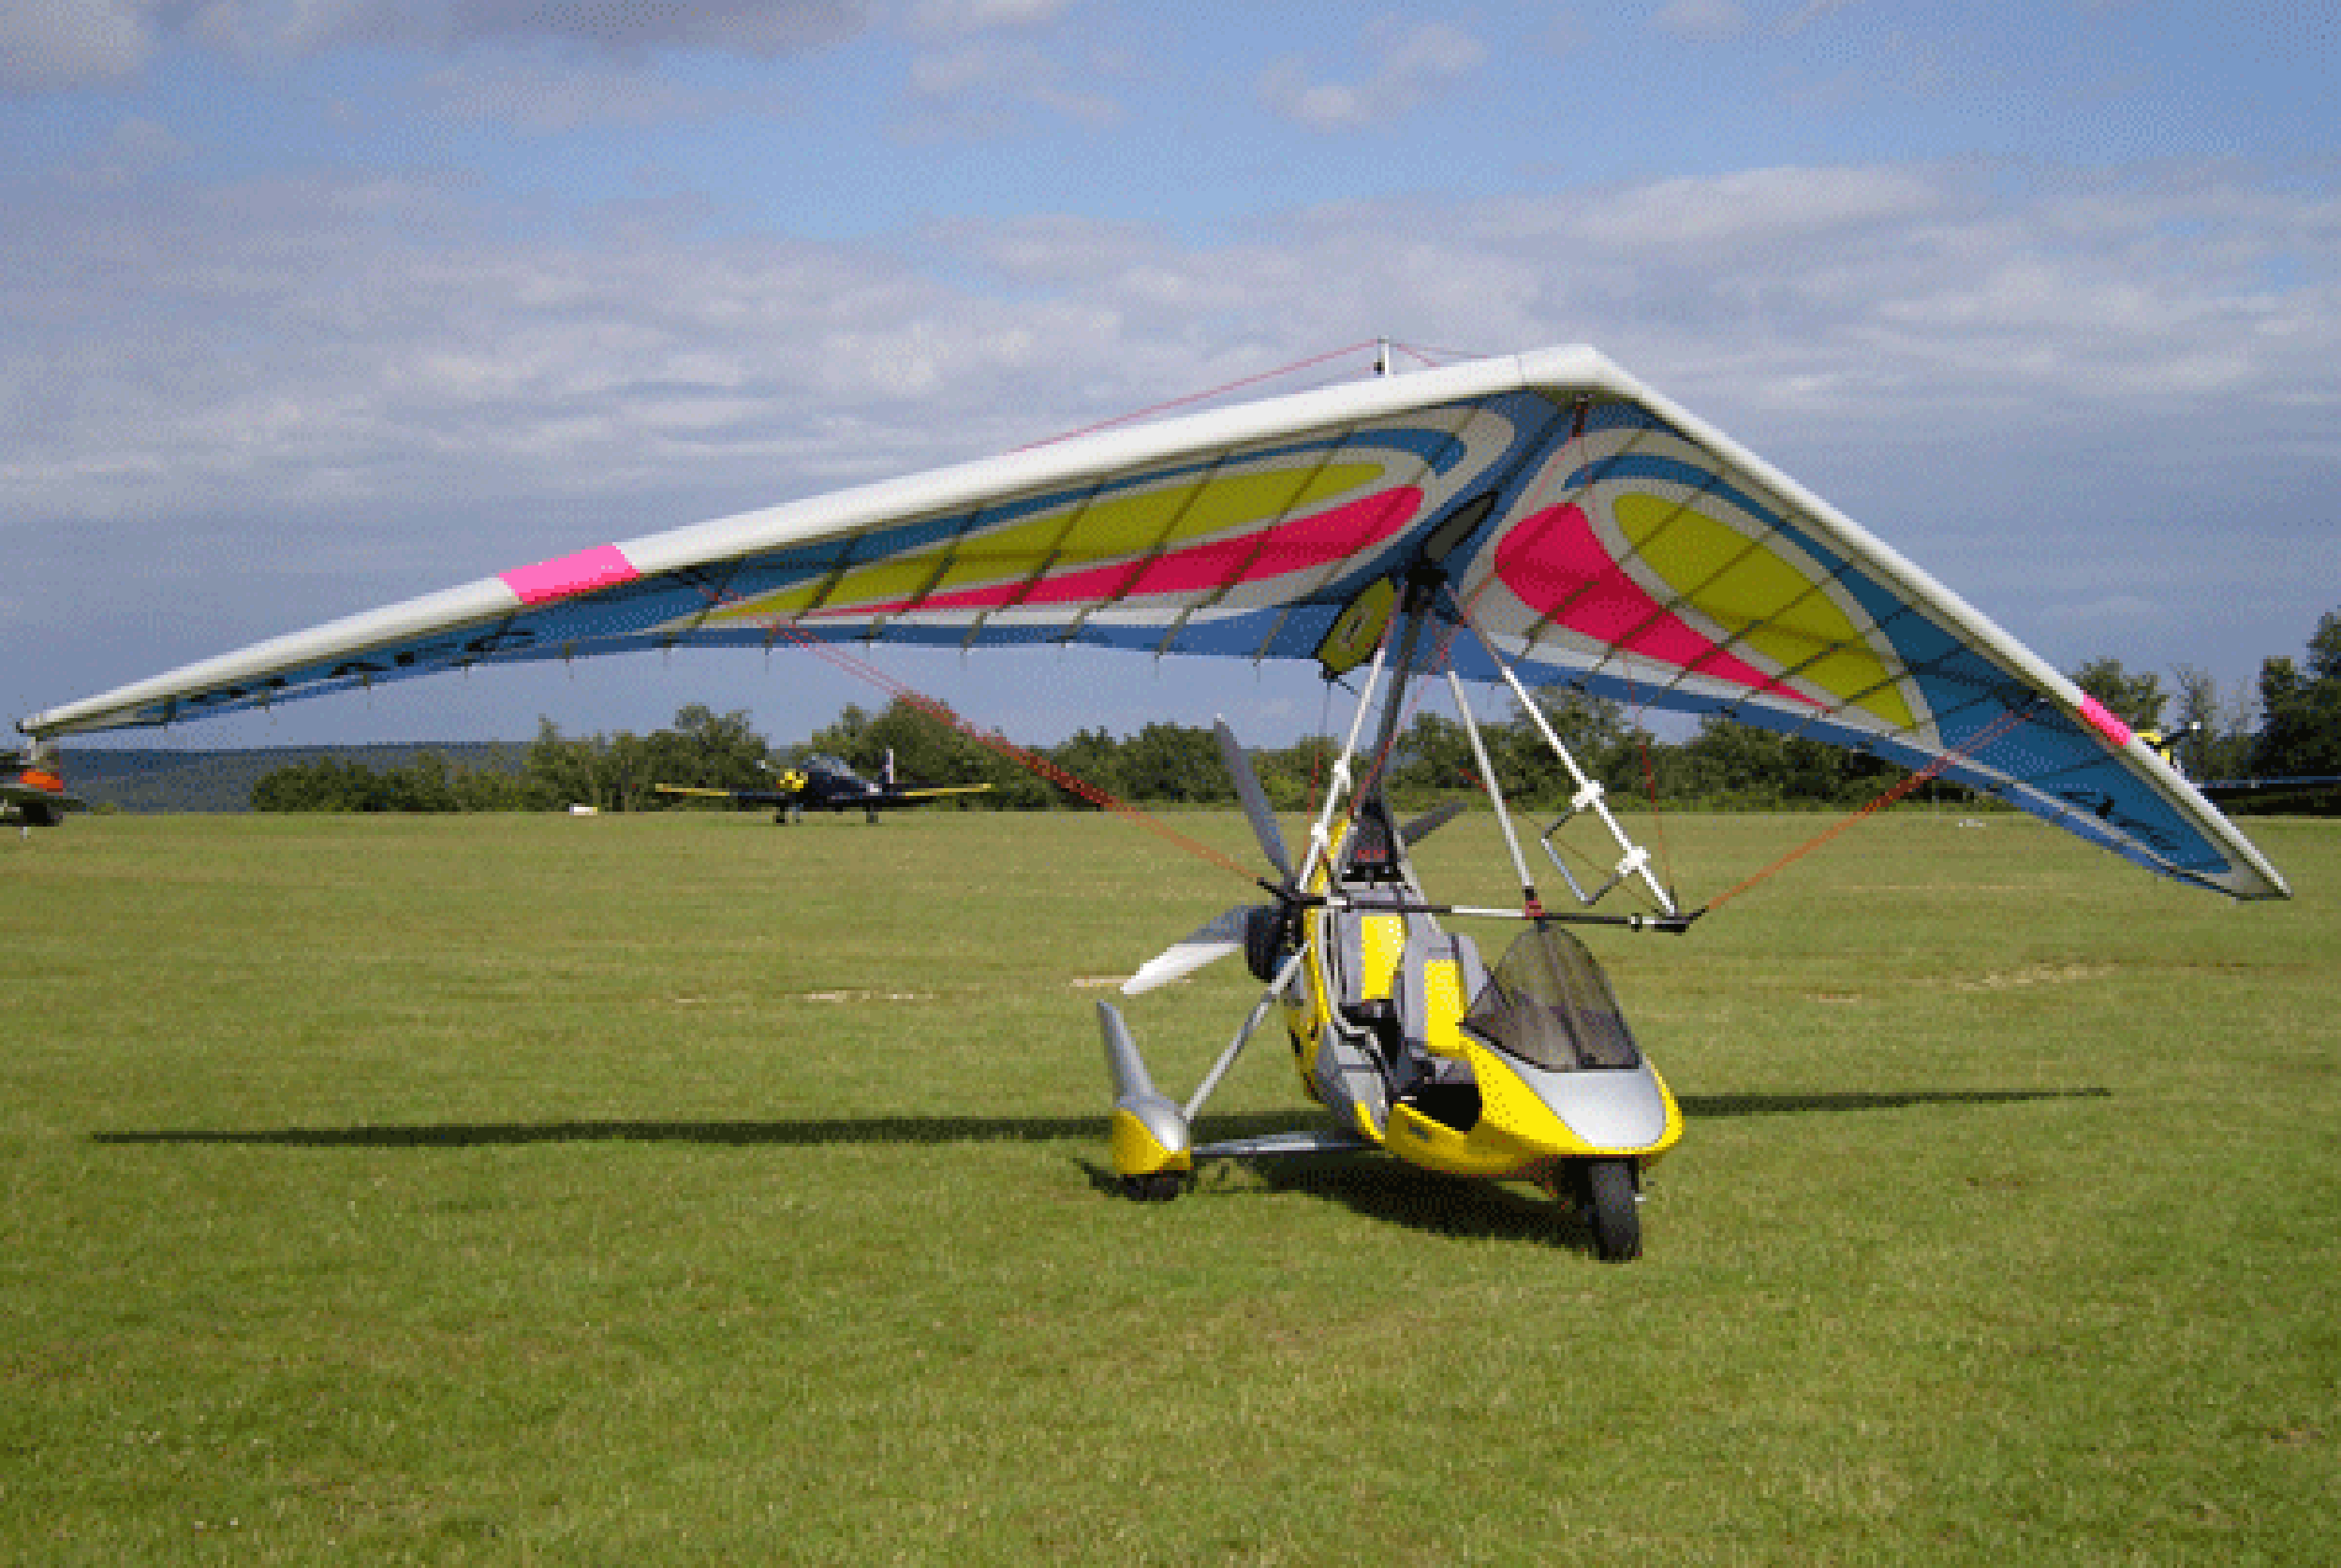
\includegraphics[height=3cm]{images/ulm} &
  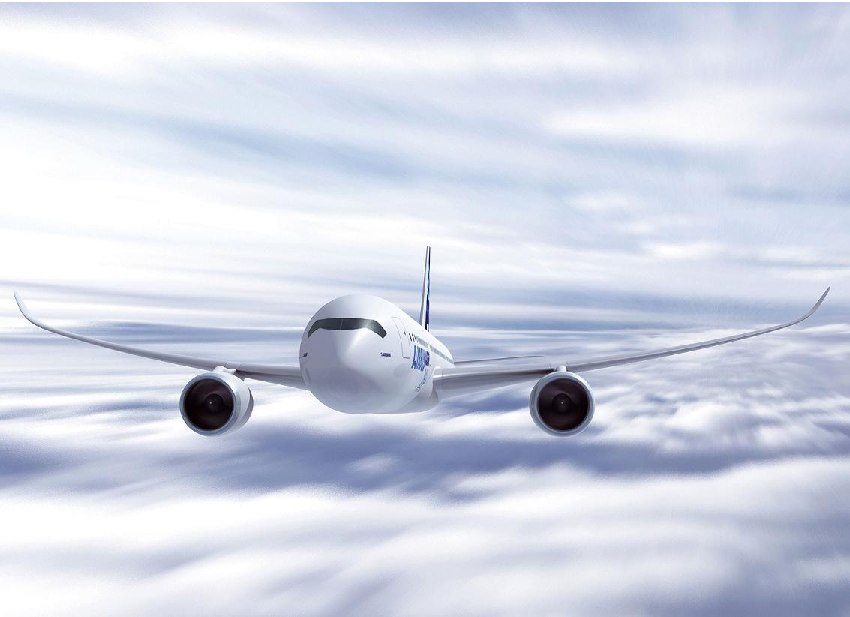
\includegraphics[height=3cm]{images/a350} \\
  Système manuel & Système mécanisé & Système automatisé \\
  \textit{Machine volante de De Vinci} & \textit{ULM} & \textit{Avion -- Airbus
A350}
 \end{tabular}
\end{center}
\end{exemple}



Réaliser un système automatisé c'est concevoir un système capable d'effectuer une ou plusieurs opérations sans intervention d'un opérateur humain. 

Les systèmes automatisés ont plusieurs objectifs : 
\paragraph*{Améliorer la sécurité}
\begin{minipage}[c]{0.7\textwidth}
 Les systèmes automatisés permettent de réaliser des opérations qui peuvent
s'avérer trop dangereuses pour les hommes. Ainsi ont-été conçu des systèmes
pour envoyer des satellites dans l'espace, pour inspecter les bassins de
combustibles dans les centrales nucléaires, pour assurer l'entretien sur des
monuments \textit{etc.}
\end{minipage}\hfill
\begin{minipage}[c]{0.2\textwidth}
 \begin{center}
 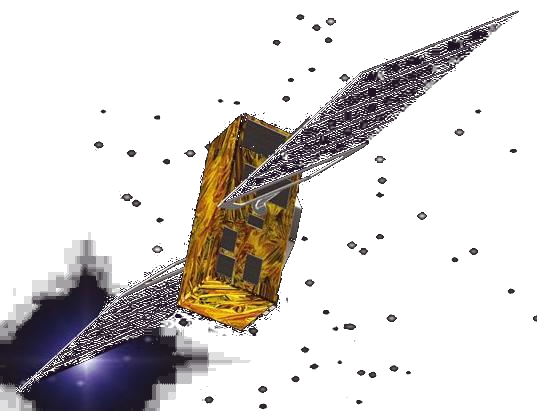
\includegraphics[height=3cm]{images/satellite}
 \end{center}
\end{minipage}

\paragraph*{Améliorer le confort}
\begin{minipage}[c]{0.7\textwidth}
Afin d'améliorer le quotidien des hommes aussi bien dans leur vie personnelle
que professionnelle, les entreprises développent des produits qui permettent de
faire évoluer notre confort : régulateur de vitesse, aspirateurs robotisés, ...
\end{minipage}\hfill
\begin{minipage}[c]{0.2\textwidth}
 \begin{center}
 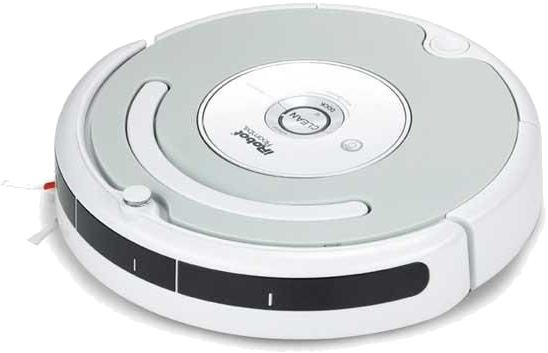
\includegraphics[height=2.5cm]{images/aspi}
 \end{center}
\end{minipage}

\paragraph*{Améliorer la qualité}
\begin{minipage}[c]{0.7\textwidth}
Dans le but d'améliorer la qualité des opérations réalisées par les hommes, des
robots chirurgicaux et d'autres produits sont en cours de développement. Ils
assurent ainsi la précision, la stabilité et la reproductibilité d'opérations
de précision.
\end{minipage}\hfill
\begin{minipage}[c]{0.2\textwidth}
 \begin{center}
 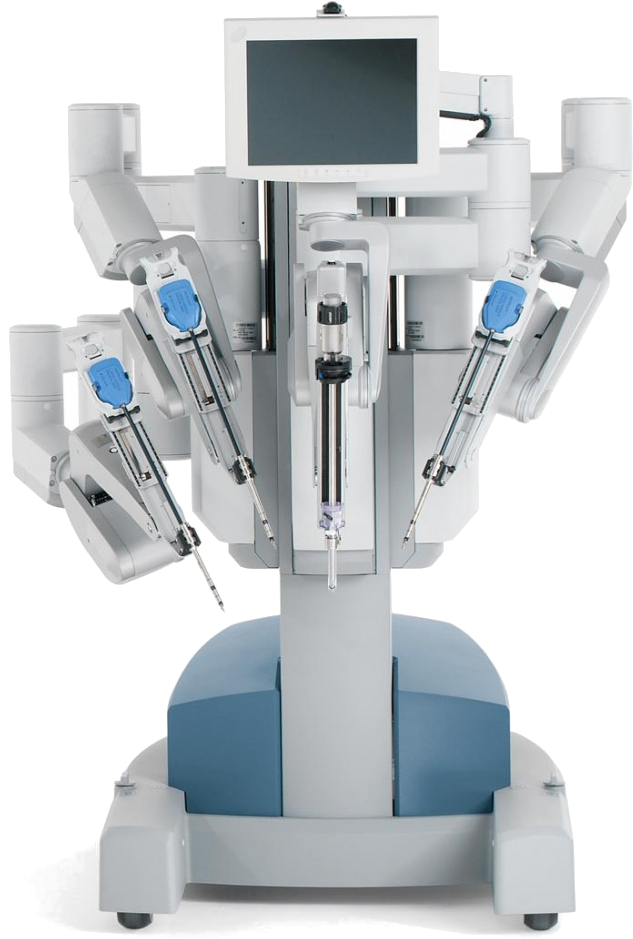
\includegraphics[height=3cm]{images/robot_chir.png}
 \end{center}
\end{minipage}

\paragraph*{Améliorer la productivité}

\begin{minipage}[c]{0.6\textwidth}
Pour améliorer la productivité industrielle et diminuer les tâches trop
répétitives pour les hommes, les chaînes de
fabrication et d'assemblage ont été largement automatisées et robotisées.
\end{minipage}\hfill
\begin{minipage}[c]{0.3\textwidth}
 \begin{center}
 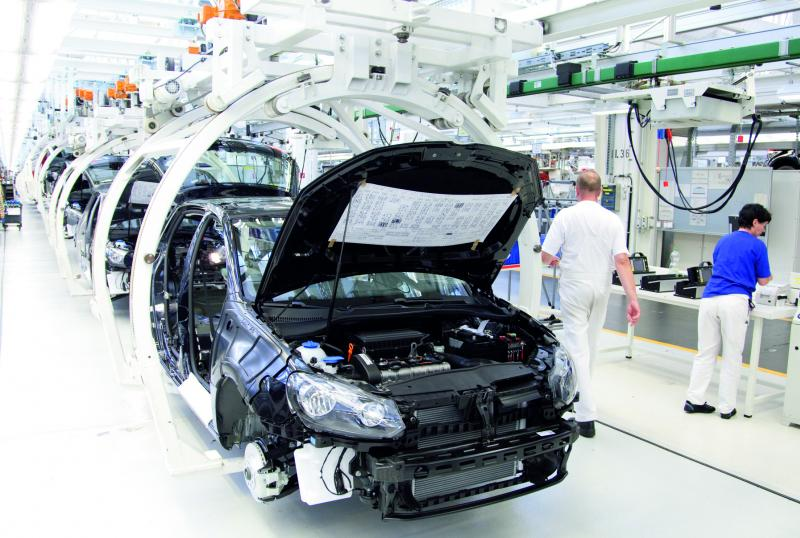
\includegraphics[height=3cm]{images/chaine_prod.png}
 \end{center}
\end{minipage}

\subsection{Définitions}


\begin{defi}  \textbf{Systèmes à logique combinatoire}

\begin{minipage}[c]{0.55\linewidth}
Les fonctions de sorties $S_j$ ne dépendent que des entrées $E_i$ à l'instant
considéré. $E_i$ et $S_j$ sont respectivement des variables et des fonctions
binaires ne pouvant prendre que les valeurs $0$ et $1$ par convention.
\end{minipage} \hfill
\begin{minipage}[c]{0.4\linewidth}
 \begin{center}
    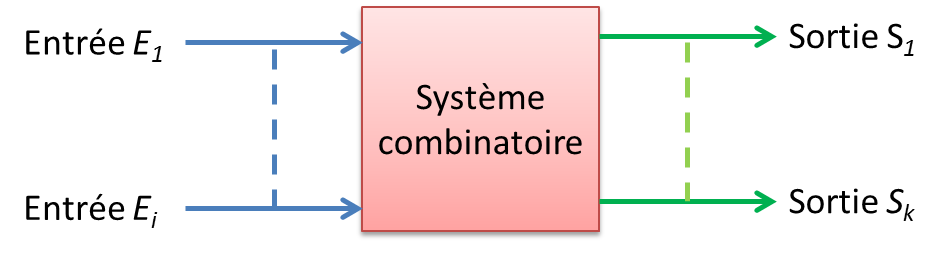
\includegraphics[width=\textwidth]{images/comb}
  \end{center}
\end{minipage}
\end{defi} 





L'outil mathématique rigoureux permettant de représenter et traiter de tels
systèmes est \textbf{l'algèbre de Boole}. Ces systèmes ont un comportement de
type \textbf{logique combinatoire}.


\begin{exemple}
 Afficheurs 7 segments
\end{exemple}



\begin{defi} \textbf{Systèmes à logique séquentielle}

\begin{minipage}[c]{0.55\linewidth}
Si une même combinaison des variables d'entrée peut donner deux sorties
différentes, il faut tenir compte de l'état du système à l'instant $t$. On
s'intéresse à ce système en le faisant évoluer séquence par séquence d'un état
fini à un autre. L'état précédent conditionnant l'état présent et ainsi de
suite. Un tel système est dit à comportement séquentiel. 
\end{minipage} \hfill
\begin{minipage}[c]{0.4\linewidth}
 \begin{center}
    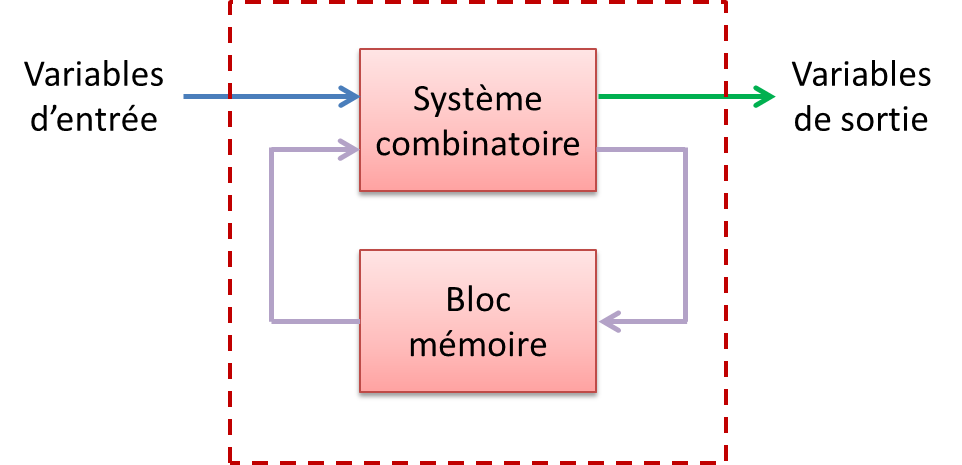
\includegraphics[width=\textwidth]{images/seq}
  \end{center}
\end{minipage}

\end{defi} 

Avec de tels systèmes, toutes les situations sont envisagées. Les événements
prévus perturbateurs du cycle entraînent, dans la plupart des cas l'arrêt de
l'automatisme (les états successifs répétitifs et prévus sont momentanément
arrêtés). Les outils généralement utilisés pour décrire et analyser ces
systèmes sont le \textbf{GRAFCET} ou les diagrammes SysML (diagramme d'état ou diagramme d'activités).

\begin{exemple}
 Ligne d'assemblage automatisée
\end{exemple}

\begin{defi}
\textbf{Systèmes automatiques ou asservis}

%\ifthenelse{\boolean{prof}}{%
Un système asservi est commandé par \textbf{une (ou des) entrée(s)} qu'il
transforme en \textbf{grandeur(s) de sortie}.
Les entrées sont de deux types : 
\begin{itemize}
 \item la loi de consigne $e(t)$ est une grandeur de commande qui est
modifiable;
\item la perturbation : c'est une entrée parasite qui nuit au bon
fonctionnement du système. On ne peut pas modifier les perturbations.
\end{itemize}

La sortie $s(t)$ est une grandeur \textbf{observable} (par des capteurs) qui
permet de juger de la qualité de la tâche accomplie.
%}{
%\rotatebox{90}{
%\begin{tabular}{p{5cm}}
%\\
%\end{tabular}}
%}
\end{defi} 

 \begin{center}
    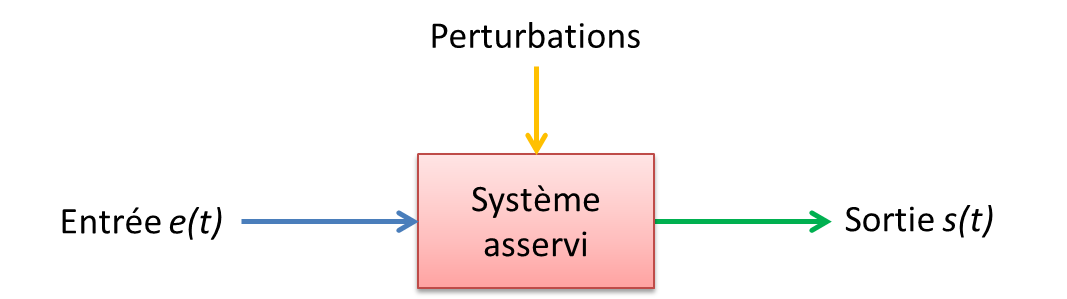
\includegraphics[width=.6\textwidth]{images/asservi}
  \end{center}
	

\begin{exemple}
Pilote automatique d'avion

 \begin{center}
    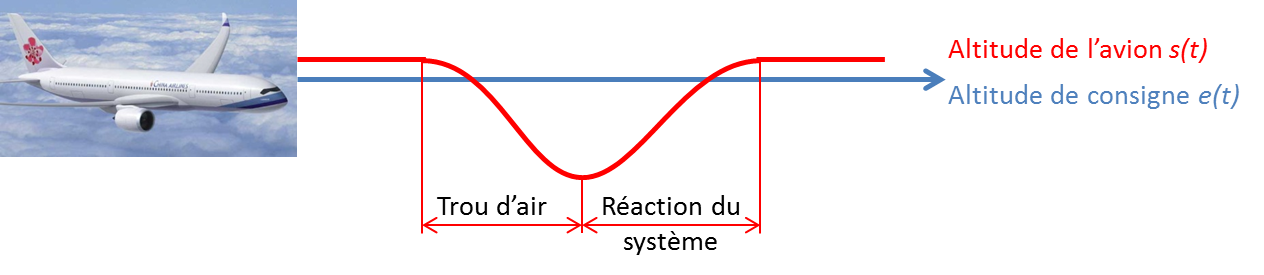
\includegraphics[width=.8\textwidth]{images/piloteauto}
  \end{center}
\end{exemple}



\subsection{Nature des informations}

\begin{defi}
 \textit{\textsf{Informations logiques}}

%\ifthenelse{\boolean{prof}}{
%\rotatebox{90}{
%\begin{tabular}{p{3cm}}
%\\
%\end{tabular}}
%}

\end{defi}

\begin{defi}
\textbf{Informations analogiques}

%\ifthenelse{\boolean{prof}}{
%\rotatebox{90}{
%\begin{tabular}{p{3cm}}
%\\
%\end{tabular}}
%}

\end{defi}


\begin{defi}
 \textbf{Informations numériques}

%\ifthenelse{\boolean{prof}}{
%\rotatebox{90}{
%\begin{tabular}{p{3cm}}
%\\
%\end{tabular}}
%}

\end{defi}


\begin{exemple}
  \begin{center}
    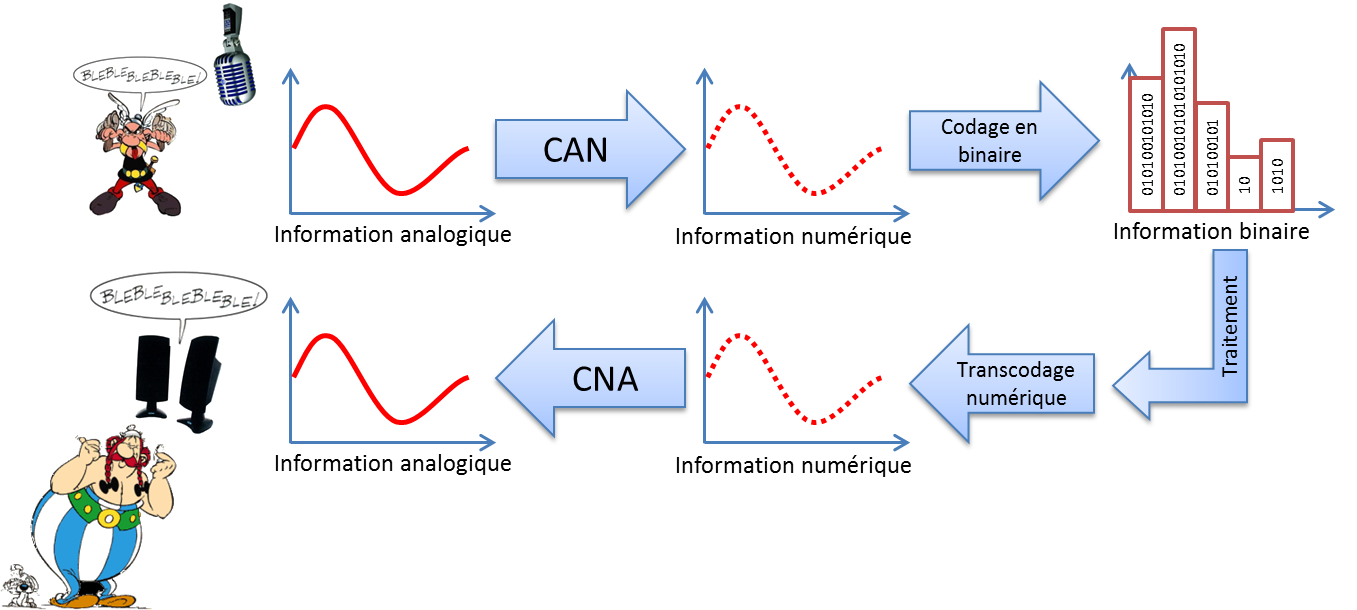
\includegraphics[width=.9\textwidth]{images/info}
  \end{center}
\end{exemple}




\section{Structure des systèmes asservis}

%\subsection{Définitions}
%\begin{defi}
% \textit{\textsf{Systèmes Linéaires Continus Invariants -- SLCI}}
%
%Les systèmes que nous utiliserons auront les propriétés suivantes :
%\begin{itemize}
%\item linéaire :
%\item continus :
%\item invariants :
%\end{itemize}
%\end{defi}

\begin{defi}
\textbf{Systèmes suiveurs}

Dans le cas de ces systèmes, la consigne $e(t)$ fluctue au cours du temps. Le système doit faire son possible pour qu'à chaque instant la cible soit suivie.
\end{defi}

\begin{exemple}

\begin{minipage}[c]{.5\textwidth}
 \begin{itemize}
\item Centres d'usinage
\item Radars
\end{itemize}
\end{minipage}
\hfill
\begin{minipage}[c]{.3\textwidth}
\begin{center}
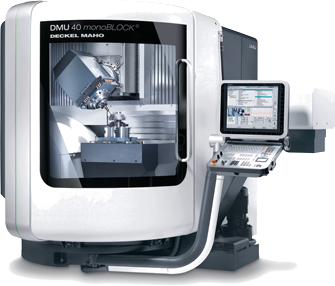
\includegraphics[width=\textwidth]{images/ugv.png}
\end{center}
\end{minipage}
\end{exemple}

\begin{defi}
\textbf{Systèmes régulateurs}

Ces systèmes ont la propriété d'avoir une consigne constante. Les perturbations font varier la position du système. Il doit donc de façon automatique revenir à la position pilotée.
\end{defi}

\begin{exemple}
 \begin{itemize}
\item régulateur de vitesse
\item réseau pneumatique
\end{itemize}
\end{exemple}

\subsection{Structure en blocs}
Dans le but de modéliser les structures asservies, on utilise une représentation en schéma blocs.

\subsubsection*{Les flèches}

\begin{minipage}[c]{.7\linewidth}
Les flèches symbolisent des grandeurs physiques. Suivant leurs positions dans le système, la grandeur physique peut être :
\begin{itemize}
\item un tension (en $V$);
\item une position (en $m$ ou en $rad$);
\item une vitesse (en $m\cdot s^{-1}$ ou en $rad\cdot s^{-1}$);
\item une accélération (en $m\cdot s^{-2}$ ou en $rad\cdot s^{-2}$);
\item un effort (en $N$);
\item ...
\end{itemize}
L'orientation de la flèche à une importance dans le fonctionnement du système.
\end{minipage}\hfill
\begin{minipage}[c]{.2\linewidth}
\begin{center}
    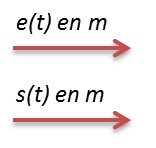
\includegraphics[width=.7\textwidth]{images/fleche2}
\end{center}
\end{minipage}

\subsubsection*{Les blocs}

Les blocs peuvent représenter des composants d'un système (actionneur, moteur, capteur, engrenage ...) ou des opérations mathématiques (dérivation ou intégration). Les blocs sont reliés par des flèches. Ils peuvent transformer la nature des grandeurs physiques. Ainsi, un moteur transforme une tension (en $V$) en une vitesse de rotation (en $rad/s$).

\begin{center}
    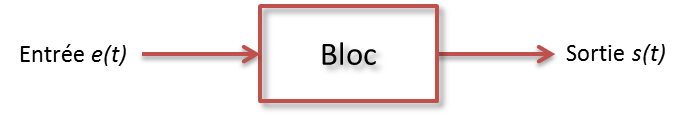
\includegraphics[width=.7\textwidth]{images/bloc}
\end{center}

\subsubsection*{Les comparateurs}
\begin{minipage}[c]{.55\linewidth}
Ils permettent d'additionner ou de soustraire des grandeurs physiques. Il est indispensable que ce soit des grandeurs de même type à chaque borne d'un comparateur. Suivant les cas on utilise des sommateurs ou des soustracteurs.
\end{minipage}\hfill
\begin{minipage}[c]{.4\linewidth}
\begin{center}
    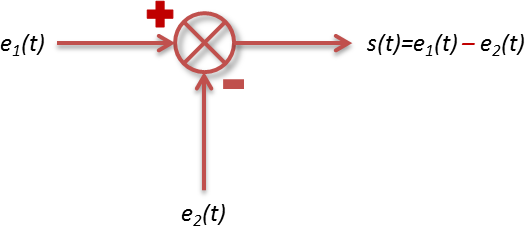
\includegraphics[width=\textwidth]{images/comp}
\end{center}
\end{minipage}

\subsubsection*{Les points de prélèvement}

\begin{minipage}[c]{.55\linewidth}
Ils permettent de réutiliser des grandeurs dans plusieurs blocs.
\end{minipage}\hfill
\begin{minipage}[c]{.4\linewidth}
\begin{center}
    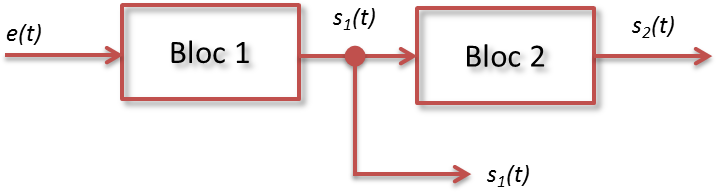
\includegraphics[width=\textwidth]{images/prel}
\end{center}
\end{minipage}

\subsection{Schéma bloc}
Le schéma bloc permet de modéliser un système complexe en tenant compte de son aspect multi physique. Communément, un système asservi prend la forme suivante : 

\begin{center}
    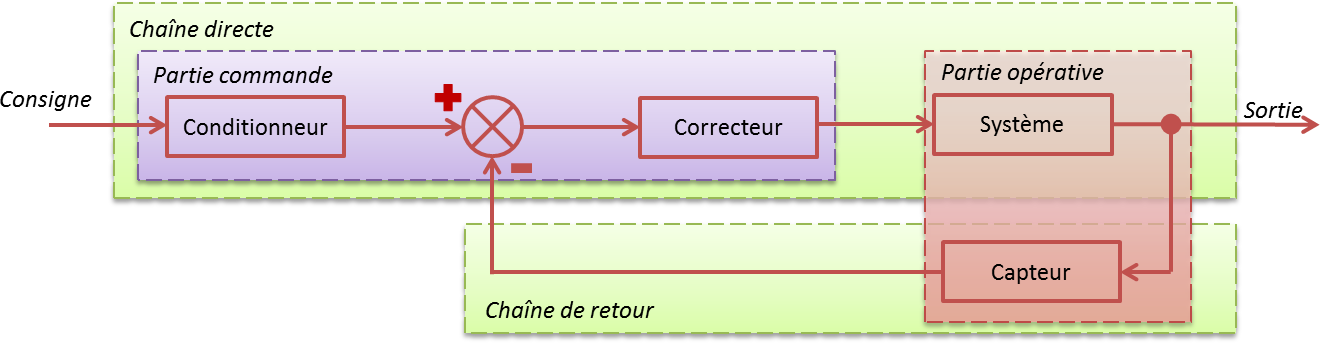
\includegraphics[width=\textwidth]{images/schbloc}
\end{center}


La caractéristique principale d'un système asservi est la présence de la chaîne de retour. C'est cette partie du système qui permet au système de respecter la consigne fixée par l'utilisateur.

\begin{exemple}
\textit{Système asservi -- schéma blocs}
\begin{center}
    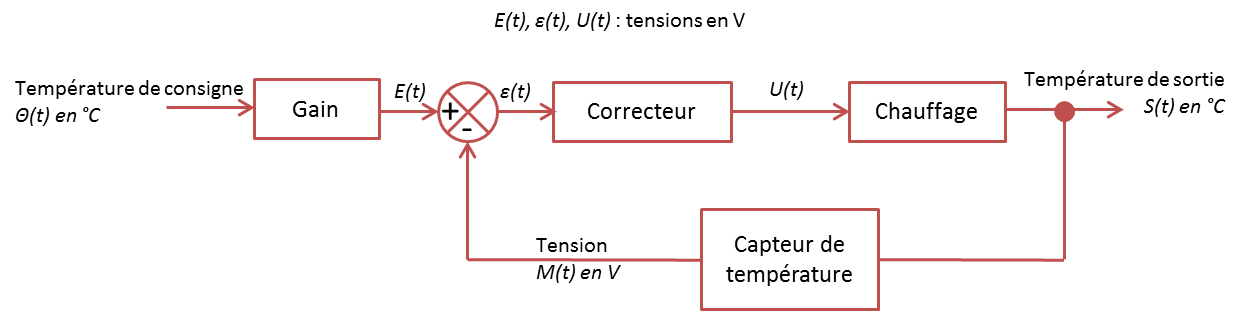
\includegraphics[width=\textwidth]{images/chauffage}
\end{center}
\end{exemple}

\newpage 

\begin{exemple}
\textit{Asservissement d'un niveau d'eau}
\begin{center}
    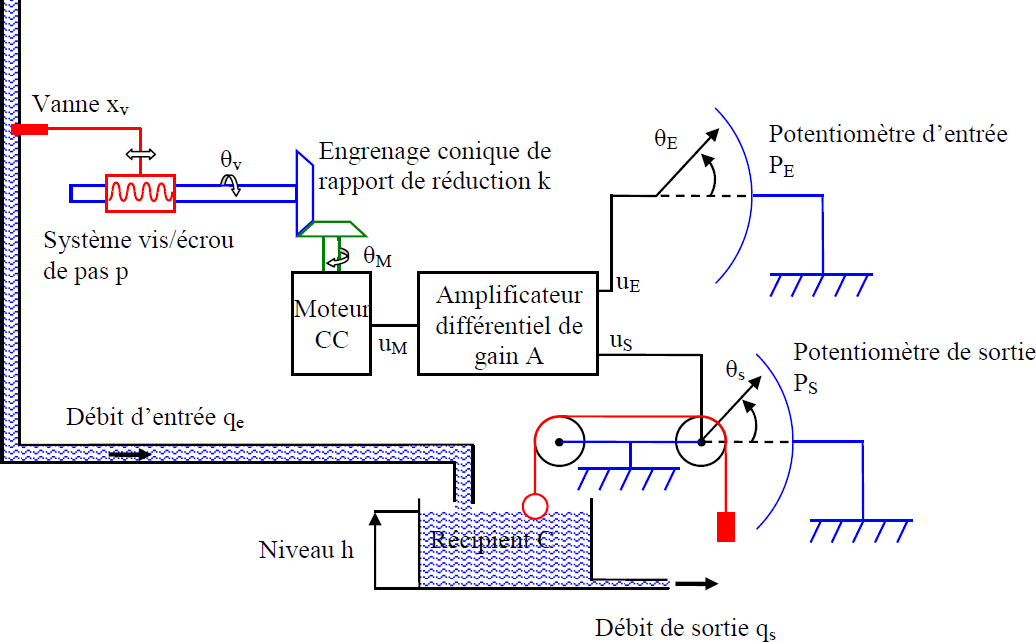
\includegraphics[width=\textwidth]{images/Exo3_01}
\end{center}

Le système représenté ci-dessus est destiné à asservir le niveau $h$ d'un liquide contenu dans un récipient $C$ pour un angle de référence $\theta_E$ réglé par l'opérateur.

Le niveau $h$ est transformé en un angle $\theta_S$ au moyen d'un flotteur agissant sur le curseur d'un potentiomètre $P_S$ $\left(\dfrac{\theta_S}{h}=K_\theta=1\;rad/m\right)$. Les deux potentiomètres $P_E$ et $P_S$, identiques, transforment les angles d'entrée et de sortie en tensions électriques dont la différence est amplifiée par un amplificateur de gain $A$. La tension de sortie de l'amplificateur $u_M$ est appliquée à l'induit d'un moteur à courant continu dont l'inducteur est alimenté par une tension constante. Ce moteur agit par l'intermédiaire d'un réducteur et d'un système vis/écrou, sur une vanne linéaire qui commande le débit $Q_E$ du liquide entrant dans le récipient $C$. Le débit de sortie $q_S$ est supposé proportionnel au niveau $h$ du liquide. 

\textit{Représenter le schéma-bloc fonctionnel du système asservi.}

\ifthenelse{\boolean{prof}}{%
\begin{center}
    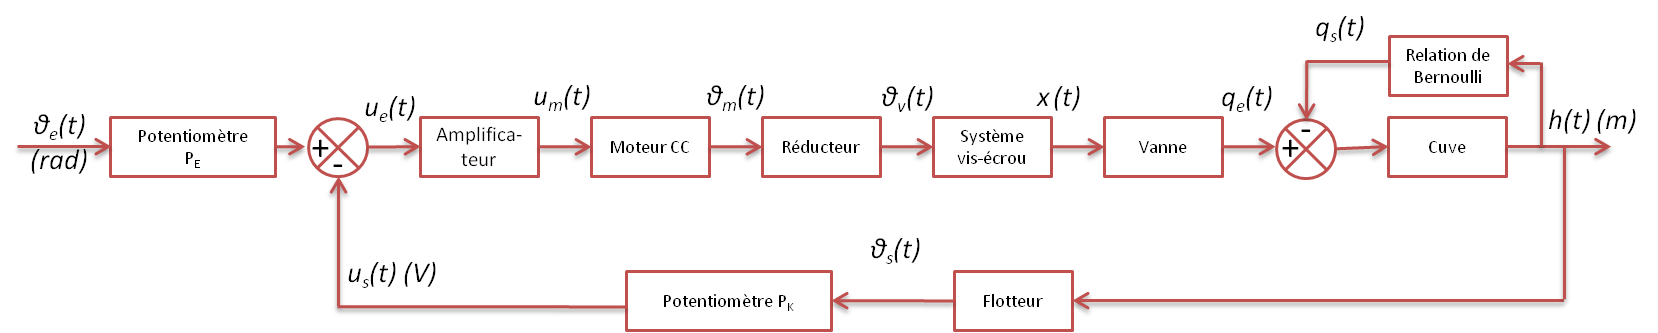
\includegraphics[width=\textwidth]{images/corrige_niveau}
\end{center}
}{%
\rotatebox{90}{%
\begin{tabular}{p{7cm}}
 \\\end{tabular}
}}
\end{exemple}

\section{Performance des systèmes asservis}
Dans l'analyse des systèmes asservis, nous distinguerons \textbf{l'aspect
statique} et \textbf{l'aspect dynamique}. 

\textbf{L'aspect statique} concerne l'étude des systèmes asservis en régime
permanent (entrée fixe). On définit l'erreur statique comme la différence entre
la sortie demandée et la sortie réalisée lorsque le régime d'équilibre est
atteint. Au cours de la synthèse des systèmes asservis, on s'efforcera en
général d'annuler cette erreur statique. 

\textbf{L'aspect dynamique}, essentiel en automatique, s'étudie par les notions
de précision dynamique, de rapidité et de stabilité. Il s'intéresse au
comportement transitoire de la sortie, soit à la suite d'une variation de la
consigne, soit de l'apparition d'une perturbation dans la chaîne d'action. 

\subsection{Précision des systèmes}
La précision qualifie l'aptitude d'un système à atteindre l'erreur visée. 

Elle est caractérisée par l'écart entre la valeur visée et la valeur
effectivement atteinte par la grandeur de sortie. L'écart éventuel s'exprime
dans la même unité que la grandeur de sortie. 


\begin{defi}
\textbf{Précision -- Écart statique $\varepsilon_S$}

\begin{minipage}[c]{0.7\textwidth}

%\ifthenelse{\boolean{prof}}{
%\rotatebox{90}{
%\begin{tabular}{p{3cm}}
%\\
%\end{tabular}}
%}
\end{minipage}\hfill
\begin{minipage}[c]{0.2\textwidth}
 \begin{center}
 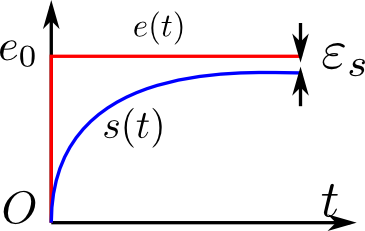
\includegraphics[width=\textwidth]{images/precision_stat}
 \end{center}
\end{minipage}

\end{defi}



\begin{defi}
\textbf{Précision -- Écart dynamique  $\varepsilon_V$}

\begin{minipage}[c]{0.7\textwidth}
%\ifthenelse{\boolean{prof}}{
%\rotatebox{90}{
%\begin{tabular}{p{3cm}}
%\\
%\end{tabular}}
%}
\end{minipage}\hfill
\begin{minipage}[c]{0.2\textwidth}
 \begin{center}
 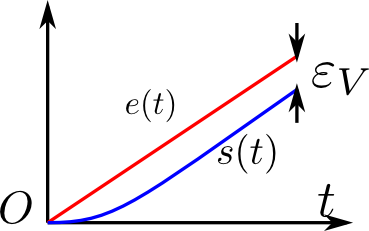
\includegraphics[width=\textwidth]{images/precision_dyn}
 \end{center}
\end{minipage}

\end{defi}


\subsection{Rapidité des systèmes}
%\begin{minipage}[c]{0.7\textwidth}
\begin{defi}
\textbf{Rapidité}

%\ifthenelse{\boolean{prof}}{
%\rotatebox{90}{
%\begin{tabular}{p{3cm}}
%\\
%\end{tabular}}
%}

\end{defi}

%\end{minipage}\hfill
%\begin{minipage}[c]{0.2\textwidth}
 \begin{center}
 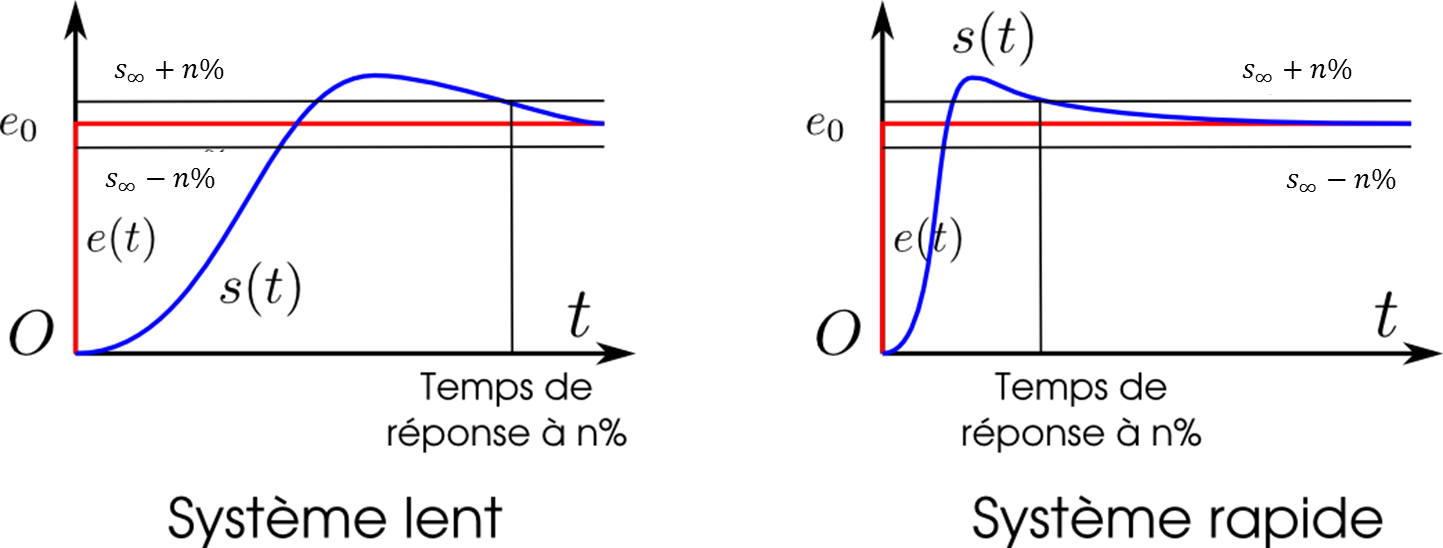
\includegraphics[width=.8\textwidth]{images/rapidite}
 \end{center}
%\end{minipage}

La valeur finale étant souvent atteinte de manière asymptotique, on retient
alors comme critère d'évaluation de la rapidité d'un système : \textbf{le temps
de réponse à n\%}. En pratique, $n=5$. 

Le temps de réponse à 5\% est le temps mis par le système pour atteindre sa
valeur de régime permanent à $\pm$5\% près et y rester. 


\begin{resultat}
\textbf{Détermination du temps de réponse à $n\%$}

\begin{enumerate}
 \item Tracer sur le même graphe la consigne $e(t)$ et la réponse du système
$s(t)$.
\item Tracer la droite correspondant à la valeur asymptotique de $s(t)$.
\item Tracer la bande correspondant à une variation de $\pm n\%$ de la valeur
asymptotique.
\item Relever la dernière valeur à partir de laquelle $s(t)$ coupe la bande et
n'en sort plus.
\end{enumerate}
\end{resultat}

%\begin{minipage}[c]{0.7\textwidth}
\subsection{Stabilité des systèmes}
\begin{defi}
 \textbf{Stabilité}

La stabilité traduit la propriété de convergence temporelle asymptotique vers
un état d'équilibre. 
\end{defi}
%\end{minipage}\hfill
%\begin{minipage}[c]{0.2\textwidth}
 \begin{center}
 \includegraphics[width=\textwidth]{images/stabilite}
 \end{center}
%\end{minipage}
Un système peut présenter une sortie divergente soit en
raison du comportement dynamique intrinsèque du système commandé soit en raison
du bouclage. Ce comportement est intolérable pour un système asservi. Dans la
pratique la seule stabilité asymptotique n'est pas suffisante. On exigera, dans
la plupart des cas, un comportement transitoire correctement amorti.


\begin{thebibliography}{2}
\bibitem{mathurin}{Cours et TD de Florestan Mathurin -- PCSI -- MPSI -- Lycée Bellevue -- Toulouse. \url{http://florestan.mathurin.free.fr}.}
\end{thebibliography}
\end{document}
